%! Mode:: "TeX:UTF-8"
%! TEX program = xelatex
\PassOptionsToPackage{quiet}{xeCJK}
\documentclass[withoutpreface,bwprint]{cumcmthesis}
\usepackage{etoolbox}
\usepackage{titlesec} %设置标题靠左
\usepackage{listings} %利用此环境插入py代码
\BeforeBeginEnvironment{tabular}{\zihao{-5}}
\usepackage[numbers,sort&compress]{natbib}  % 文献管理宏包
\usepackage[framemethod=TikZ]{mdframed}  % 框架宏包
\usepackage{url}  % 网页链接宏包
\usepackage{pdfpages} %插入附录部分
% 三线表格式
\usepackage{booktabs}
\usepackage{adjustbox}
\usepackage{subcaption}  % 子图宏包
\newcolumntype{C}{>{\centering\arraybackslash}X}
\newcolumntype{R}{>{\raggedleft\arraybackslash}X}
\newcolumntype{L}{>{\raggedright\arraybackslash}X}
\usepackage{amsmath}
\usepackage{booktabs}
\usepackage{geometry}
\usepackage{graphicx}
\usepackage{makecell} % Include this package in the preamble

\usepackage{fancyhdr} % 导入页眉页脚宏包
\usepackage{lastpage} % 获取总页数

% 设置页眉样式
\pagestyle{fancy}
\fancyhf{} % 清空默认设置

% 自定义页眉内容
\fancyhead[L]{Team A apmcm24210022} % 左侧页眉内容
\fancyhead[R]{\makebox[0pt][r]{Page \thepage\ of 93}} % 右侧页眉内容，确保内容右对齐并与下划线右端对齐

% 自定义页眉下划线
\renewcommand{\headrulewidth}{0.4pt} % 设置页眉下划线宽度
\renewcommand{\headrule}{
    \hrule width \textwidth height 0.4pt % 设置下划线为页面宽度
}

% 删除页脚内容
\fancyfoot{} % 清空页脚内容

% 让页眉从目录后的页面开始
\usepackage{afterpage}
\newcommand{\applyheader}{
    \afterpage{
        \pagestyle{fancy} % 应用自定义页眉样式
    }
}



\usepackage[english]{babel} % 设置语言为英文
\renewcommand{\thesection}{\Roman{section}.} % 一级章节编号改为希腊数字 (I, II, III)

%代码附录部分
\usepackage{listings}
\usepackage{xcolor} % 可选：用于设置代码颜色

\lstset{ 
    basicstyle=\ttfamily,
    keywordstyle=\color{blue},
    commentstyle=\color{gray},
    stringstyle=\color{red},
    numbers=left,
    numberstyle=\tiny,
    stepnumber=1,
    numbersep=5pt,
    backgroundcolor=\color{white},
    showspaces=false,
    showstringspaces=false,
    showtabs=false,
    tabsize=2,
}

% 调整页面边距
\geometry{
    a4paper,
    left=2cm,
    right=2cm,
    top=2cm,
    bottom=2cm
}


% 定义部分section标题靠左的命令
\newcommand{\leftalignedsection}[1]{%
    \section*{#1}%
    \addcontentsline{toc}{section}{#1}%
}

% 使用titlesec包设置部分section标题靠左
\titleformat{name=\section,numberless}[block]{\raggedright\bfseries\Large}{}{0pt}{}

\usepackage{graphicx}
\usepackage{amsmath}
\usepackage{geometry}
\usepackage{array}
\usepackage{makecell}

%%%%%%%%%%%%%%%%%%%%%%%%%%%%%%%%%%%%%%%%%%%%%%%%%%%%%%%%%%%%%
%% 正文
\begin{document}

\begin{center}
    \begin{minipage}{0.75\textwidth}

        % 表格部分
        \begin{center}
            \renewcommand\arraystretch{1.5} % 调整行高
            \begin{tabular}{|p{0.25\linewidth}|p{0.25\linewidth}|}
                \hline
                \makecell{Team Number} & \makecell{apmcm24210022} \\ \hline
                \makecell{Problem Chosen} & \makecell{A} \\ \hline
            \end{tabular}
        \end{center}

        % 表格和下划线之间的间距
        %\vspace{0.2em} % Adjust this space as necessary
        
    \end{minipage}
\end{center}

% 下划线，设置为页面宽度
\hrule width \textwidth height 2pt % 设置下划线为页面宽度，厚度为0.4pt

% 标题部分
\begin{center}
    {\Large \textbf{A Study on Classification, Enhancement, and Scene Adaptability \\ Based on Underwater Image Degradation Models}} % 论文标题，字号可调节
\end{center}


\pagenumbering{gobble}  % 隐藏页码

\begin{abstract}

In this study, with the objective of optimizing underwater image quality and enhancing visibility in complex aquatic environments, we systematically addressed five pivotal challenges.

\textbf{For Question 1}, a degradation classification method is proposed, combining \textbf{brightness deviation analysis} via \textbf{gray-level histograms}, \textbf{clarity assessment} using the \textbf{Laplacian operator}, and \textbf{color shift detection} in the \textbf{LAB color space}. This method classifies underwater images into \textbf{color distortion}, \textbf{blurriness}, and \textbf{low contrast} categories,  It provides a computationally efficient and intuitive approach, laying the groundwork for future model design and enhancement techniques.

\textbf{For Question 2}, a degradation model based on the \textbf{McGlamery underwater light transmission model} is proposed. This model incorporates key parameters such as the \textbf{absorption coefficient}, \textbf{scattering coefficient}, and \textbf{background light intensity} to simulate light propagation and restore the image’s clarity and true color. It provides a scientific explanation for the degradation process and demonstrates strong \textbf{robustness} under varying conditions of water depth, turbidity, and background light intensity.

\textbf{For Question 3}, targeted enhancement methods are introduced: \textbf{multi-scale histogram equalization} for low-light correction, \textbf{wavelength compensation} and \textbf{contrast correction} for color restoration, and \textbf{Laplacian sharpening} for edge enhancement. The effectiveness of these methods is evaluated using performance metrics such as PSNR, UCIQE, and UIQM, showing significant improvements in specific degradation scenarios.

\textbf{For Question 4}, a fusion enhancement model is proposed, which combines \textbf{multi-dimensional weights} to adaptively enhance degraded images. By optimizing \textbf{luminance compensation}, \textbf{color correction}, and \textbf{sharpness enhancement}, this model significantly outperforms individual enhancement techniques, delivering exceptional performance in complex underwater environments.

\textbf{For Question 5}, it is \textbf{scene-specific} enhancement techniques and \textbf{single} enhancement techniques compared for complex underwater scenes. Scene-specific techniques are tailored for specific conditions, while complex scene techniques based on \textbf{deep learning}, offer greater adaptability for handling dynamic environments. Based on this, practical recommendations for underwater visual enhancement are provided, with an emphasis on selecting suitable methods for different underwater conditions.

\textbf{keywords:}{\quad Underwater Optical Model\quad  Image Degradation Classification\quad Multi-Scale Histogram Equalization\quad McGlamery\quad Laplacian Operator \quad PSNR \quad UCIQE \quad UIQM \quad }

\end{abstract}
%%%%%%%%%%%%%%%%%%%%%%%%%%%%%%%%%%%%%%%%%%%%%%%%%%%%%%%%%%%%% 

\begin{center}
    \tableofcontents  % 目录
\end{center}

\cleardoublepage  % 清除当前页面并开始新的一页
\pagenumbering{arabic}  % 从正文开始页码为 1

%%%%%%%%%%%%%%%%%%%%%%%%%%%%%%%%%%%%%%%%%%%%%%%%%%%%%%%%%%%%%  
\newpage
\applyheader

\section{Introduction}

\subsection{Background}

With the rapid advancement of technology, underwater image acquisition and processing have become vital tools in deep-sea exploration, marine biology, and ocean engineering. However, the challenging underwater environment significantly degrades image quality, leading to issues such as reduced clarity, low contrast, and color distortion, which hinder visual perception and information extraction. Light absorption and scattering in water weaken different wavelengths, with red and green light being more attenuated, causing a dominant blue-green tint. Furthermore, scattering caused by suspended particles further reduces image resolution and detail, posing challenges for both human observation and automated processing algorithms.

Underwater image enhancement has emerged as a key research focus, aiming to improve visual quality, clarity, and color fidelity. This involves addressing the complex optical properties of water through signal processing, image enhancement, and deep learning techniques. Traditional methods based on physical models analyze light absorption and scattering mechanisms to restore image quality. However, these models often struggle in complex underwater scenarios. In contrast, deep learning approaches, leveraging large datasets, can automatically learn image features and improve restoration, but their performance is limited in data-scarce or highly variable environments. Thus, combining physical models with data-driven techniques to develop adaptable enhancement methods is a primary research direction.

Future advancements in underwater image enhancement will integrate optical modeling and deep learning to enhance algorithm robustness and generalization, enabling effective application across diverse environments. This integration will improve the visual fidelity of underwater images and provide reliable support for marine science and engineering applications, laying the foundation for future advancements in underwater vision technology.

\begin{figure}[htbp]
    \centering
    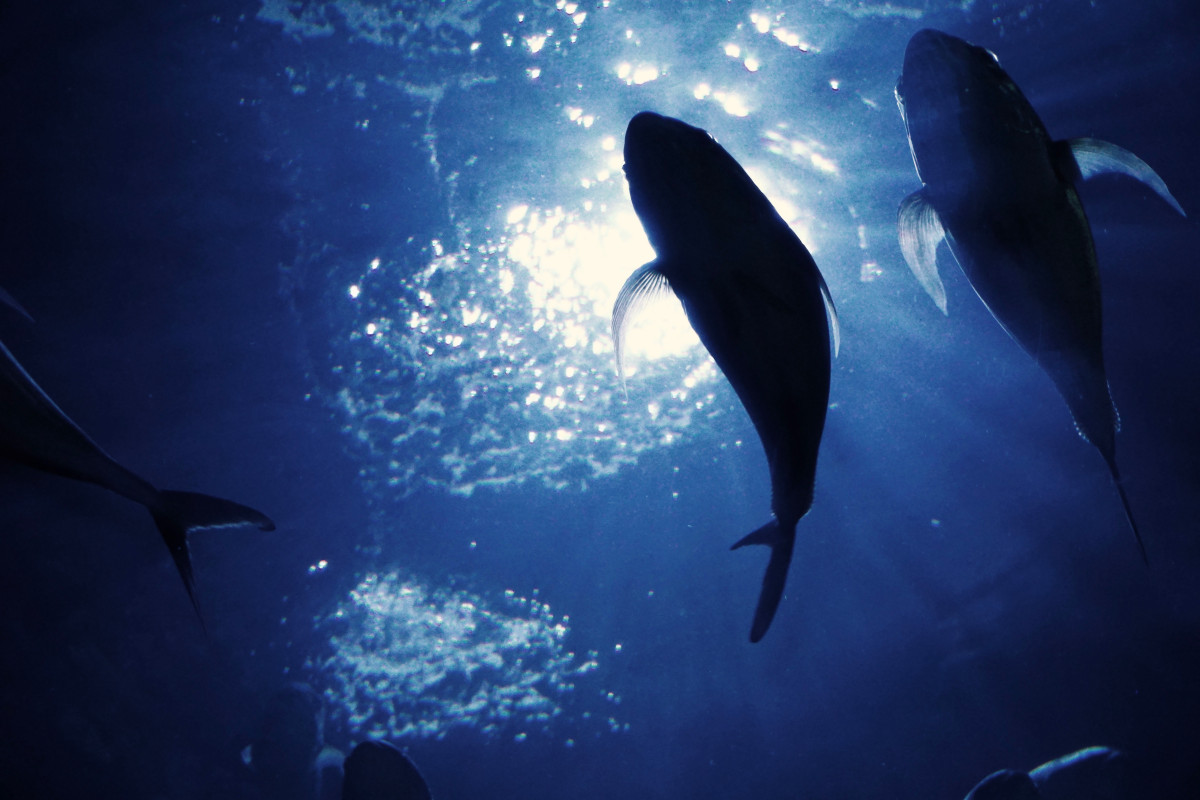
\includegraphics[width=0.6\linewidth]{figures_plus/微信图片_20241123231709.jpg}
    \caption{}
    \label{fig:enter-label}
\end{figure}

\subsection{Restatement of the Question}

\subsubsection{Question 1: Classification and Feature Analysis of Underwater Image Degradation}

The first Question focuses on analyzing the degradation characteristics of underwater images. It requires categorizing images into three classes: color distortion, blurriness, and low contrast, based on their degradation features. The task involves identifying the causes and characteristics of degradation. Specifically, statistical analysis is to be performed on the underwater images provided in \textbf{Attachment 1}, explaining the mechanisms behind the observed degradation phenomena. The classification results should be documented in the provided table in the attachment.

\subsubsection{Question 2: Construction and Analysis of Underwater Image Degradation and Restoration Models}

The second Question centers on constructing a restoration model for degraded images based on the physical model of underwater imaging. Restoration analysis should be conducted for different types of degradation, aiming to recover image sharpness, color, and contrast. The focus is on evaluating the rationality of the restoration model and its applicability under various degradation characteristics.

\subsubsection{Question 3: Design of Underwater Image Enhancement Methods for Specific Scenarios}

The third Question targets designing an effective underwater image enhancement method tailored to specific scenarios. The method's effectiveness should be validated using the provided dataset. By calculating image quality metrics such as \textbf{PSNR}, \textbf{UCIQE}, and \textbf{UIQM}, the performance of various enhancement methods is to be compared, with an analysis of their strengths and weaknesses.

\subsubsection{Question 4: Adaptability and Performance Evaluation of Enhancement Models in Complex Scenarios}

The fourth Question aims to propose an underwater image enhancement model suitable for complex scenarios. The adaptability and performance of the proposed model should be validated through experiments. Using the image data in \textbf{Attachment 2}, the enhanced images should be evaluated using quality metrics, and the model's performance in various scenarios should be analyzed. A summary of its applicability is also required.
%%%%%%%%%%%%%%%%%%%%%%%%%%%%%%%%%%%%%%%%%%%%%%%%%%%%%%%%%%%%% 
\newpage
\section{Question Analysis}

\subsection{Analysis of Question 1}

The optical complexity of underwater environments causes image degradation, such as color distortion, blurring, and low contrast. This task aims to classify the underwater images into three categories: color distortion, blurring, and low contrast, identifying the characteristics and causes of each. The analysis includes calculating luminance deviation using the grayscale histogram, assessing sharpness with the Laplacian operator's variance, detecting color distortion via LAB color space statistics, and applying threshold-based classification for quick and intuitive analysis. The classification results provide data support for subsequent restoration and enhancement.

\subsection{Analysis of Question 2}

Underwater image degradation is primarily due to light absorption and scattering. This task utilizes the McGlamery underwater light transmission model to restore degraded images by calculating light transmittance using absorption and scattering coefficients and simulating the degradation process with background light. The restoration method adjusts parameters like water depth, turbidity, and light intensity, and verifies the model’s effectiveness across different degradation types. The goal is to restore image clarity, contrast, and color fidelity while analyzing the model's limitations and potential improvements.

\subsection{Analysis of Poblem 3}

Image enhancement methods must address specific degradation features. This task proposes methods for low luminance, color distortion, and blurring: Multi-Scale Histogram Equalization (MSHE) improves brightness in low-light conditions; wavelength compensation restores color fidelity for color distortion; and Laplacian sharpening enhances edge details for blurring. The effectiveness of these methods is evaluated using PSNR, UCIQE, and UIQM metrics, providing a basis for comparing performance across different scenarios.

\subsection{Analysis of Question 4}

In complex underwater scenes, multiple degradation factors affect image quality, requiring a comprehensive enhancement approach. This task introduces a fusion model that combines color correction and contrast enhancement to address multiple types of degradation. The model uses multi-weight fusion strategies to optimize enhancement effects by adjusting various weights (e.g., Laplacian contrast, saliency). Experiments with the dataset from Attachment 2 validate the model's ability to enhance brightness, color, and clarity, and analyze its performance across different complex scenes.

%%%%%%%%%%%%%%%%%%%%%%%%%%%%%%%%%%%%%%%%%%%%%%%%%%%%%%%%%%%%% 
\newpage
\section{Model Preparation}

\subsection{Model Assumptions}

To simplify the Question and simulate real-world conditions, the following assumptions are made:

\begin{itemize}[itemindent=2em]

\item \textbf{Uniform Water Body Assumption:} The optical properties of the water (e.g., absorption and scattering coefficients) are uniformly distributed and constant throughout the research area.

\item \textbf{Single Light Source Assumption:} The underwater scene is illuminated by a single, stable light source, with no consideration of multiple overlapping sources.

\item \textbf{Uniform Background Light Assumption:} Background light intensity is constant across depth and position, simplifying modeling.

\item \textbf{No Lens Distortion Assumption:} The imaging equipment is assumed to be free of optical distortion, ensuring that image geometry is unaffected by the water medium.

\item \textbf{No Dynamic Factors Assumption:} Dynamic factors such as waves or currents are neglected, assuming a static scene.

\item \textbf{Pixel Independence Assumption:} Image degradation is assumed to be independent for each pixel, allowing for pixel-by-pixel processing.

\end{itemize}

\subsection{Description of the Symbol}

The key mathematical symbols used in this paper are listed in Table 1.

\begin{table}[htbp]
\centering
\begin{tabular}{@{}>{\centering\arraybackslash}p{4cm}>{\centering\arraybackslash}p{10cm}@{}}
\toprule
\textbf{Symbol} & \textbf{Description} \\ 
\midrule
$J_t(x)$ & Clear image representing direct light from the target scene. \\ 
$N$ & Total number of pixels in the image, calculated as width $\times$ height. \\ 
$I_{\text{blurred}}(x, y)$ & Original clear image. \\ 
$B_{\infty}$ & Background light intensity, representing the contribution of scattered light. \\ 
$t_t(x)$ & Transmission rate of light, calculated as $\exp(-C(\lambda) \cdot r)$. \\ 
$C(\lambda)$ & Light attenuation coefficient, defined as $C(\lambda) = a(\lambda) + b(\lambda)$. \\ 
$h(x, y)$ & Point spread function (PSF), modeling the blurring effects. \\ 
\bottomrule
\end{tabular}
\caption{}
\end{table}

%%%%%%%%%%%%%%%%%%%%%%%%%%%%%%%%%%%%%%%%%%%%%%%%%%%%%%%%%%%%% 
\newpage
\section{Establishment and Solution of the Model for Question 1}

In Question 1, the objective is to analyze the underwater images in Attachment 1 and classify them into three categories: Colorcast, Low Light, and Blur. The first step involves visually inspecting the images to understand their characteristics and degradation patterns. This visual assessment forms the basis for subsequent statistical analysis and classification, enabling the identification and quantification of specific distortions.

\begin{figure}[htbp]
    \centering
    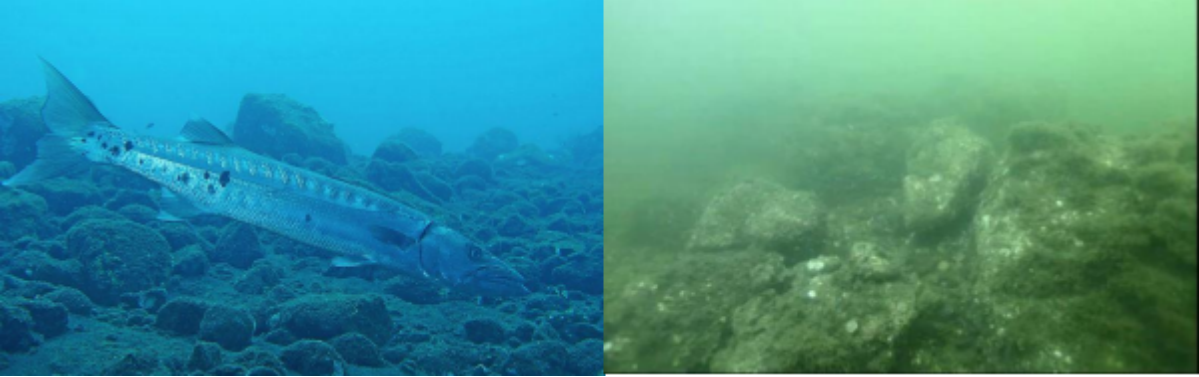
\includegraphics[width=0.75\linewidth]{figures_plus/微信图片_20241123231717.png}
    \caption{}
    \label{fig:enter-label}
\end{figure}

By observing the images in the attachment (Attachment1,image\_001, image\_002), we can identify the following possible visual characteristics:

\textbf{Colorcast:}

A shift in color balance, with a dominant blue, green, or other color bias, caused by differential light absorption and scattering in underwater environments, leading to uneven color distribution.

 \textbf{Low Light:}

Reduced brightness and loss of detail in darker regions, indicating insufficient lighting due to limited light penetration in underwater settings, which affects image clarity and contrast.

\textbf{Blur:}

 Indistinct edges and lack of fine detail, indicative of blurriness caused by scattering, camera shake, or focus issues, resulting in diminished sharpness.

These characteristics were identified through visual inspection and aligned with the classification criteria for Colorcast, Low Light, and Blur.

\begin{figure}[htbp]
    \centering
    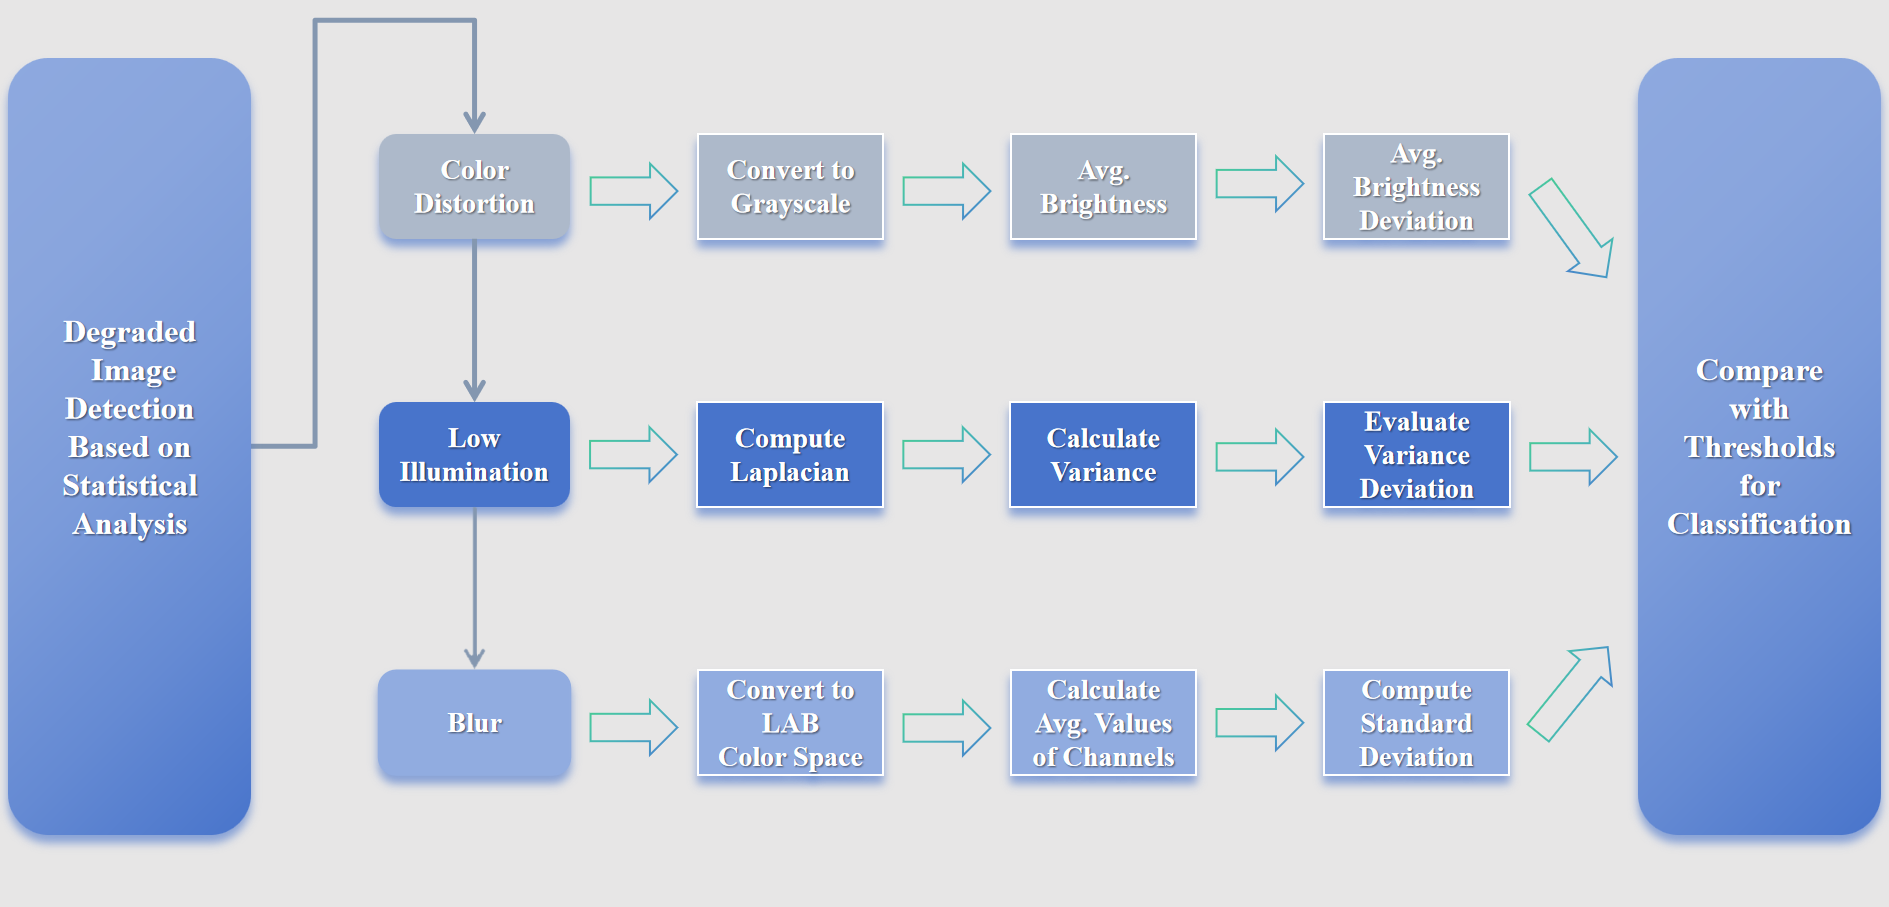
\includegraphics[width=0.75\linewidth]{figures_plus/微信图片_20241123231722.png}
    \caption{}
    \label{fig:enter-label}
\end{figure}

\subsection{Brightness Detection}

\subsubsection{Grayscale Conversion of the Image}

For brightness detection, converting the RGB color image to grayscale is essential, as pixel values in a grayscale image directly represent brightness. In contrast, an RGB image contains three channels—Red, Green, and Blue—each encoding both brightness and color information. Grayscale conversion simplifies brightness quantification by removing the influence of color.

The formula for grayscale conversion is:
\[\text{Gray} = 0.299 \cdot R + 0.587 \cdot G + 0.114 \cdot B \]

Where $R$ , $G$, and $B$ represent the red, green, and blue channel values of a pixel, respectively. The weights are determined based on human visual sensitivity to these colors. After converting an image from the RGB space to the grayscale space, each pixel value ranges from 0 to 255, where 0 represents the lowest brightness and 255 represents the highest. This preprocessing step provides a unified data format for subsequent brightness detection.

\subsubsection{Global Brightness Deviation Calculation}

The brightness mean deviation $d_a$ measures the deviation of the overall image brightness from $128$ (the midpoint of the grayscale range). The calculation formula is:
\[d_a = \frac{1}{N} \sum_{i=1}^{N} (x_i - 128)\]


\subsubsection{Absolute Global Brightness Deviation Calculation}

To eliminate the effects of positive and negative deviations canceling each other out, the absolute value of the brightness deviation (\( D \)) is calculated:
\[D = |d_a|\]

This metric represents the overall deviation degree of brightness, regardless of whether the image is too bright or too dark.

\subsubsection{Weighted Histogram-Based Brightness Deviation Calculation}

To account for the non-uniform distribution of brightness in the image, a weighted brightness deviation $M_a$ is computed using the grayscale histogram $\text{Hist}[i]$ :
\[M_a = \frac{1}{N} \sum_{i=0}^{255} (i - 128) \cdot \text{Hist}[i]\]


The absolute value of  $M_a$ , denoted as $M = |M_a|$ , is used to evaluate the global distribution characteristics of brightness deviations.

\subsubsection{Calculation of Brightness Anomaly Parameters}

The brightness anomaly parameter $k$ is defined as the ratio of overall brightness deviation $D$ to the distribution deviation $M$:
\[k = \frac{D}{M}\]


The parameter $k$ determines whether the image brightness is normal:

\begin{itemize}[itemindent=2em]
    \item If $k < 1$ , the image brightness is normal, indicating ideal lighting conditions.

    \item If  $k \geq 1$ , the image exhibits abnormal brightness, which may be excessively bright or dark.
\end{itemize}

Furthermore, analyzing the brightness deviation direction can determine the specific nature of the anomaly:

\begin{itemize}[itemindent=2em]
    \item  If $d_a > 0$ : The image is too bright, potentially caused by excessive lighting or background light interference, leading to overexposed regions with loss of detail.

    \item  If $d_a < 0$ : The image is too dark, likely due to insufficient lighting or severe attenuation of light in water, causing target details to be hidden or blurred.
\end{itemize}

\subsection{Fuzzy Detection}

Image sharpness is a key metric for evaluating edge details and texture information. In digital image processing, blurred images typically lack high-frequency details and exhibit weaker edge responses, whereas sharp images contain rich edge information and high-frequency components. To assess sharpness, we use the Laplacian Variance Method\textsuperscript{\cite{he2005laplacian}}, which quantifies the high-frequency response of an image by calculating its variance. This method provides a fast and effective means for detecting blurred images. The principle, formula, and implementation steps are outlined below.

\subsubsection{Laplacian Operator}

The Laplacian operator is a second-order differential operator commonly used for edge detection in image processing. It calculates the gradient intensity of brightness changes, highlighting high-frequency regions such as edges and textures. For a given image I(x,y), the Laplacian operator\textsuperscript{\cite{ratcliffe1997damage}} is mathematically defined as:
\[L(x, y) = \frac{\partial^2 I(x, y)}{\partial x^2} + \frac{\partial^2 I(x, y)}{\partial y^2}\]

Where:

\begin{itemize}[itemindent=2em]
    \item $I(x, y)$: Grayscale value of the image at pixel position $(x, y)$,

    \item $L(x, y)$: Response value calculated using the Laplacian operator.
\end{itemize}

The output of the Laplacian operator is a new image where high-frequency regions (e.g., edges or texture details) exhibit significant non-zero responses, while low-frequency regions (e.g., flat or blurred areas) have responses close to zero. This output intuitively reflects the richness of high-frequency details in the image.

\begin{figure}[htbp]
    \centering
    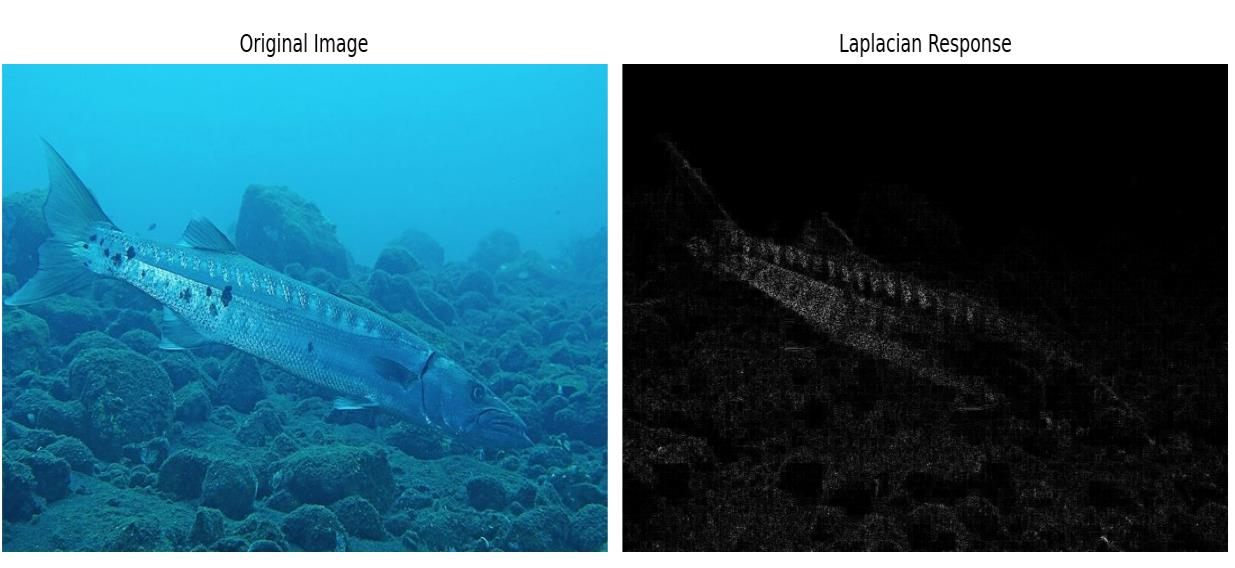
\includegraphics[width=0.75\linewidth]{figures_plus/微信图片_20241123231732.png}
    \caption{}
    \label{fig:enter-label}
\end{figure}

\subsubsection{Laplacian Variance Calculation}

To quantify the high-frequency components in an image, the variance of the Laplacian output is calculated. Variance is a key statistical metric used to measure the dispersion of data distribution, and in image processing, it reflects the range of pixel value variations. The formula for calculating Laplacian variance is:
\[\text{Var}(L) = \frac{1}{N} \sum_{i=1}^{N} (L_i - \mu)^2\]

Where:

\begin{itemize}[itemindent=2em]
    \item $L_i$: Value of the $i$-th pixel in the Laplacian output image,

    \item $\mu$: Mean of pixel values, defined as:$\mu = \frac{1}{N} \sum_{i=1}^{N} L_i$

    \item $N$: Total number of pixels in the image.
\end{itemize}

A higher variance value indicates that the image contains more high-frequency components, with richer edges and details, implying higher sharpness. Conversely, a lower variance value suggests that the image is blurred and lacks high-frequency details.

\subsubsection{Criteria for Judging Image Clarity}

Before classifying images, a sharpness threshold \( T \) must be set to determine whether an image is blurred. The criterion is as follows:
\[\text{Judgment Criterion} =
\begin{cases} 
\text{Sharp}, & \text{if } \text{Var}(L) \geq T \\ 
\text{Blurred}, & \text{if } \text{Var}(L) < T 
\end{cases}\]


The final threshold is robust and accurate, making it applicable to sharpness detection tasks for similar types of images. This provides a reliable basis for further image enhancement or blur correction.

\begin{table}[htbp]
\centering
\resizebox{0.75\textwidth}{!}{%
\begin{tabular}{@{}>{\centering\arraybackslash}p{4cm}>{\centering\arraybackslash}p{4cm}>{\centering\arraybackslash}p{4cm}@{}}
\toprule
\textbf{Image ID} & \textbf{Laplacian Variance} & \textbf{Manual Label} \\ 
\midrule
Image\_001 & 664.33 & Clear \\ 
Image\_002 & 68.93 & Blurred \\ 
Image\_003 & 116.44 & Blurred \\ 
$\vdots$   & $\vdots$   & $\vdots$ \\ 
Image\_047 & 310.55 & Clear \\ 
Image\_048 & 279.42 & Clear \\ 
Image\_049 & 127.10 & Clear \\ 
\bottomrule
\end{tabular}%
}
\caption{}
\end{table}

Through extensive statistical analysis of sample data, we determined that a Laplacian variance threshold\textsuperscript{\cite{singer2006graph}} $T$ of approximately 120 can effectively distinguish between clear and blurred images. Specifically:

\begin{itemize}[itemindent=2em]
    \item When the variance value exceeds **150**, the image typically contains abundant edge and detail information and can be classified as a **clear image**.

    \item When the variance value falls below **150**, the image exhibits a significant loss of high-frequency details, appearing in an overall **blurred state**.
\end{itemize}

The determination of this threshold involved multiple rounds of experimental validation and manual selection, ensuring its strong applicability and robustness for various image types.

\subsection{Color Shift Detection}

\begin{figure}[htbp]
    \centering
    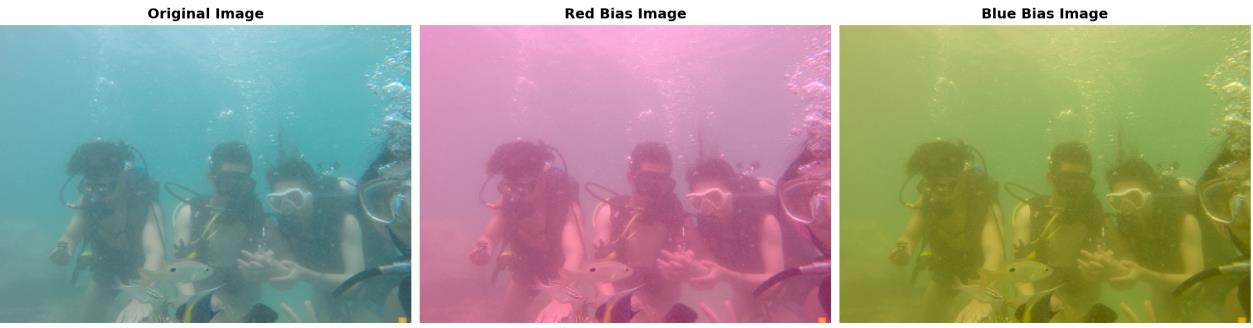
\includegraphics[width=0.75\linewidth]{figures_plus/微信图片_20241123231736.png}
    \caption{}
    \label{fig:enter-label}
\end{figure}

Color shift in an image refers to the systematic deviation of its color distribution from the expected or standard color balance. This deviation often manifests as a pronounced bias toward a particular color (e.g., red or blue), which can compromise the image's visual quality.

To quantify this color deviation, we utilize a \textbf{LAB color space-based method}. The LAB color space, which aligns closely with human color perception, consists of three components: brightness (L) and two orthogonal chromaticity components, (A) and (B), representing the green-red and blue-yellow axes, respectively. This model effectively captures and quantifies color shifts within the image.

\subsubsection{Image Color Space Conversion}

To accurately evaluate color distribution characteristics, the input image is first converted from the RGB color space to the LAB color space. In LAB:

\begin{itemize}[itemindent=2em]
    \item $L$: Brightness component,

    \item $A$: Green-Red chromaticity axis,

    \item $B$: Blue-Yellow chromaticity axis.
\end{itemize}

The LAB color space, designed based on human perception, effectively separates color and brightness information, providing a solid foundation for subsequent color shift detection. Statistical analysis of the $A$ and $B$ channels reflects the trends in color shift, supporting the calculation of average color shift and deviation assessment.

\begin{figure}[htbp]
    \centering
    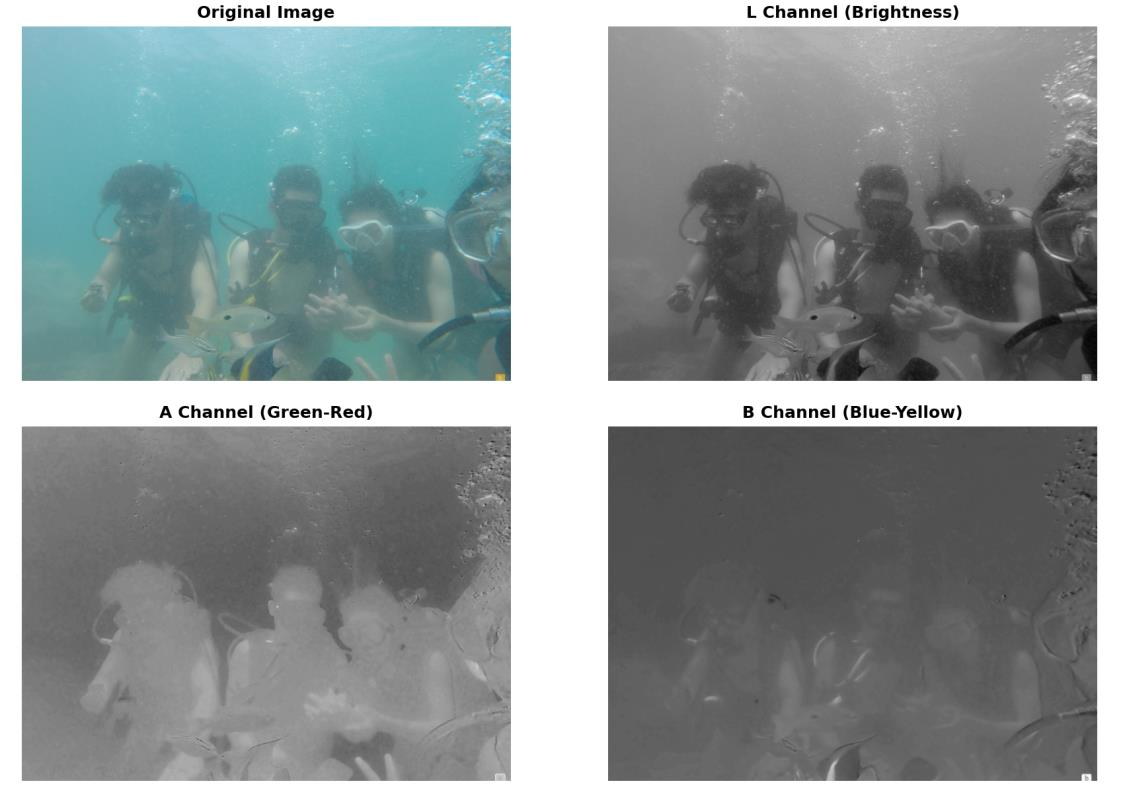
\includegraphics[width=0.75\linewidth]{figures_plus/微信图片_20241123231746.png}
    \caption{}
    \label{fig:enter-label}
\end{figure}

\subsubsection{Calculate the Average Color Shift}

The overall color shift is measured by calculating the average values of all pixels in the \( A \) and \( B \) channels. The formulas are:
\[d_a = \frac{1}{H \cdot W} \sum_{i=1}^{H} \sum_{j=1}^{W} A(i, j)\]

\[d_b = \frac{1}{H \cdot W} \sum_{i=1}^{H} \sum_{j=1}^{W} B(i, j)\]

The larger the absolute values of $d_a$ and $d_b$ , the more significant the overall color shift.

\subsubsection{Normalize Deviations}

To reflect the dispersion of color distribution, the normalized deviations for the $A$ and $B$ channels are calculated as:
\[\text{msqA} = \frac{1}{H \cdot W} \sum_{y} |y - 128 - d_a|\]

\[\text{msqB} = \frac{1}{H \cdot W} \sum_{y} |y - 128 - d_b|\]


\subsubsection{Calculate the Color Shift Ratio}

Based on the average color shift and normalized deviation, the color shift ratio $R$ is calculated as:
\[ R = \frac{\sqrt{d_a^2 + d_b^2}}{\sqrt{\text{msqA}^2 + \text{msqB}^2}}\]

where:

\begin{itemize}[itemindent=2em]
    \item The numerator measures the overall average color shift,

    \item The denominator measures the dispersion of the color distribution.
\end{itemize}

A larger $R$ value indicates more significant color shift.

\subsubsection{Criteria for Judgment}

Similar to other detection tasks, we annotate a sample dataset to identify normal or expected color standards as "non-color-shifted" and images exhibiting systematic deviations as "color-shifted." The steps include:

\textbf{Step 1:} Annotate images with normal color distribution as "non-color-shifted" and those with significant deviations as "color-shifted."

\vspace{0.5em}
\textbf{Step 2:} Calculate the color shift ratio (\( R \)) for each image to quantify the degree of color deviation.

\vspace{0.5em}
\textbf{Step 3:} Analyze the distribution of \( R \) values for "non-color-shifted" and "color-shifted" images, and identify a preliminary boundary as the candidate threshold.

\vspace{0.5em}
\textbf{Step 4:} Iteratively adjust the threshold \( T \) through testing and error analysis to ensure accurate classification of color-shifted and non-color-shifted images.


The final threshold is optimized for accuracy and robustness, ensuring its applicability to similar datasets and providing a solid foundation for further image enhancement or color correction.

\begin{table}[htbp]
\centering
\resizebox{0.75\textwidth}{!}{%
\begin{tabular}{@{}>{\centering\arraybackslash}p{5cm}>{\centering\arraybackslash}p{5cm}>{\centering\arraybackslash}p{5cm}@{}}
\toprule
\textbf{Image ID} & \textbf{Color Shift Ratio} & \textbf{Manual Label} \\ 
\midrule
Image\_001 & 1.635 & Non-color-shifted \\ 
Image\_002 & 3.25 & Non-color-shifted \\ 
Image\_003 & 2.25 & Non-color-shifted \\ 
$\vdots$   & $\vdots$   & $\vdots$ \\ 
Image\_047 & 0.85 & Non-color-shifted \\ 
Image\_048 & 1.45 & Non-color-shifted \\ 
Image\_049 & 3.85 & Non-color-shifted \\ 
\bottomrule
\end{tabular}%
}
\caption{}
\end{table}

Based on the experiments and statistical analysis, we set the threshold for the color shift ratio as $T = 4$ . The judgment criteria are defined as follows:
\[\text{Classification} =
\begin{cases} 
\text{Color-shifted}, & R > T \\
\text{Non-color-shifted}, & R \leq T
\end{cases}\]

%%%%%%%%%%%%%%%%%%%%%%%%%%%%%%%%%%%%%%%%%%%%%%%%%%%%%%%%%%%%%
\newpage
\section{Building and Solving the Model of Question 2}

The complexity and instability of light propagation in underwater environments cause significant image degradation, including reduced brightness, color distortion, and loss of sharpness. Absorption and scattering of light, along with suspended particles amplifying scattering, contribute to image blur. These issues are critical for applications like underwater exploration, marine surveying, and robotics, which depend on high-quality image data.

\begin{figure}[htbp]
    \centering
    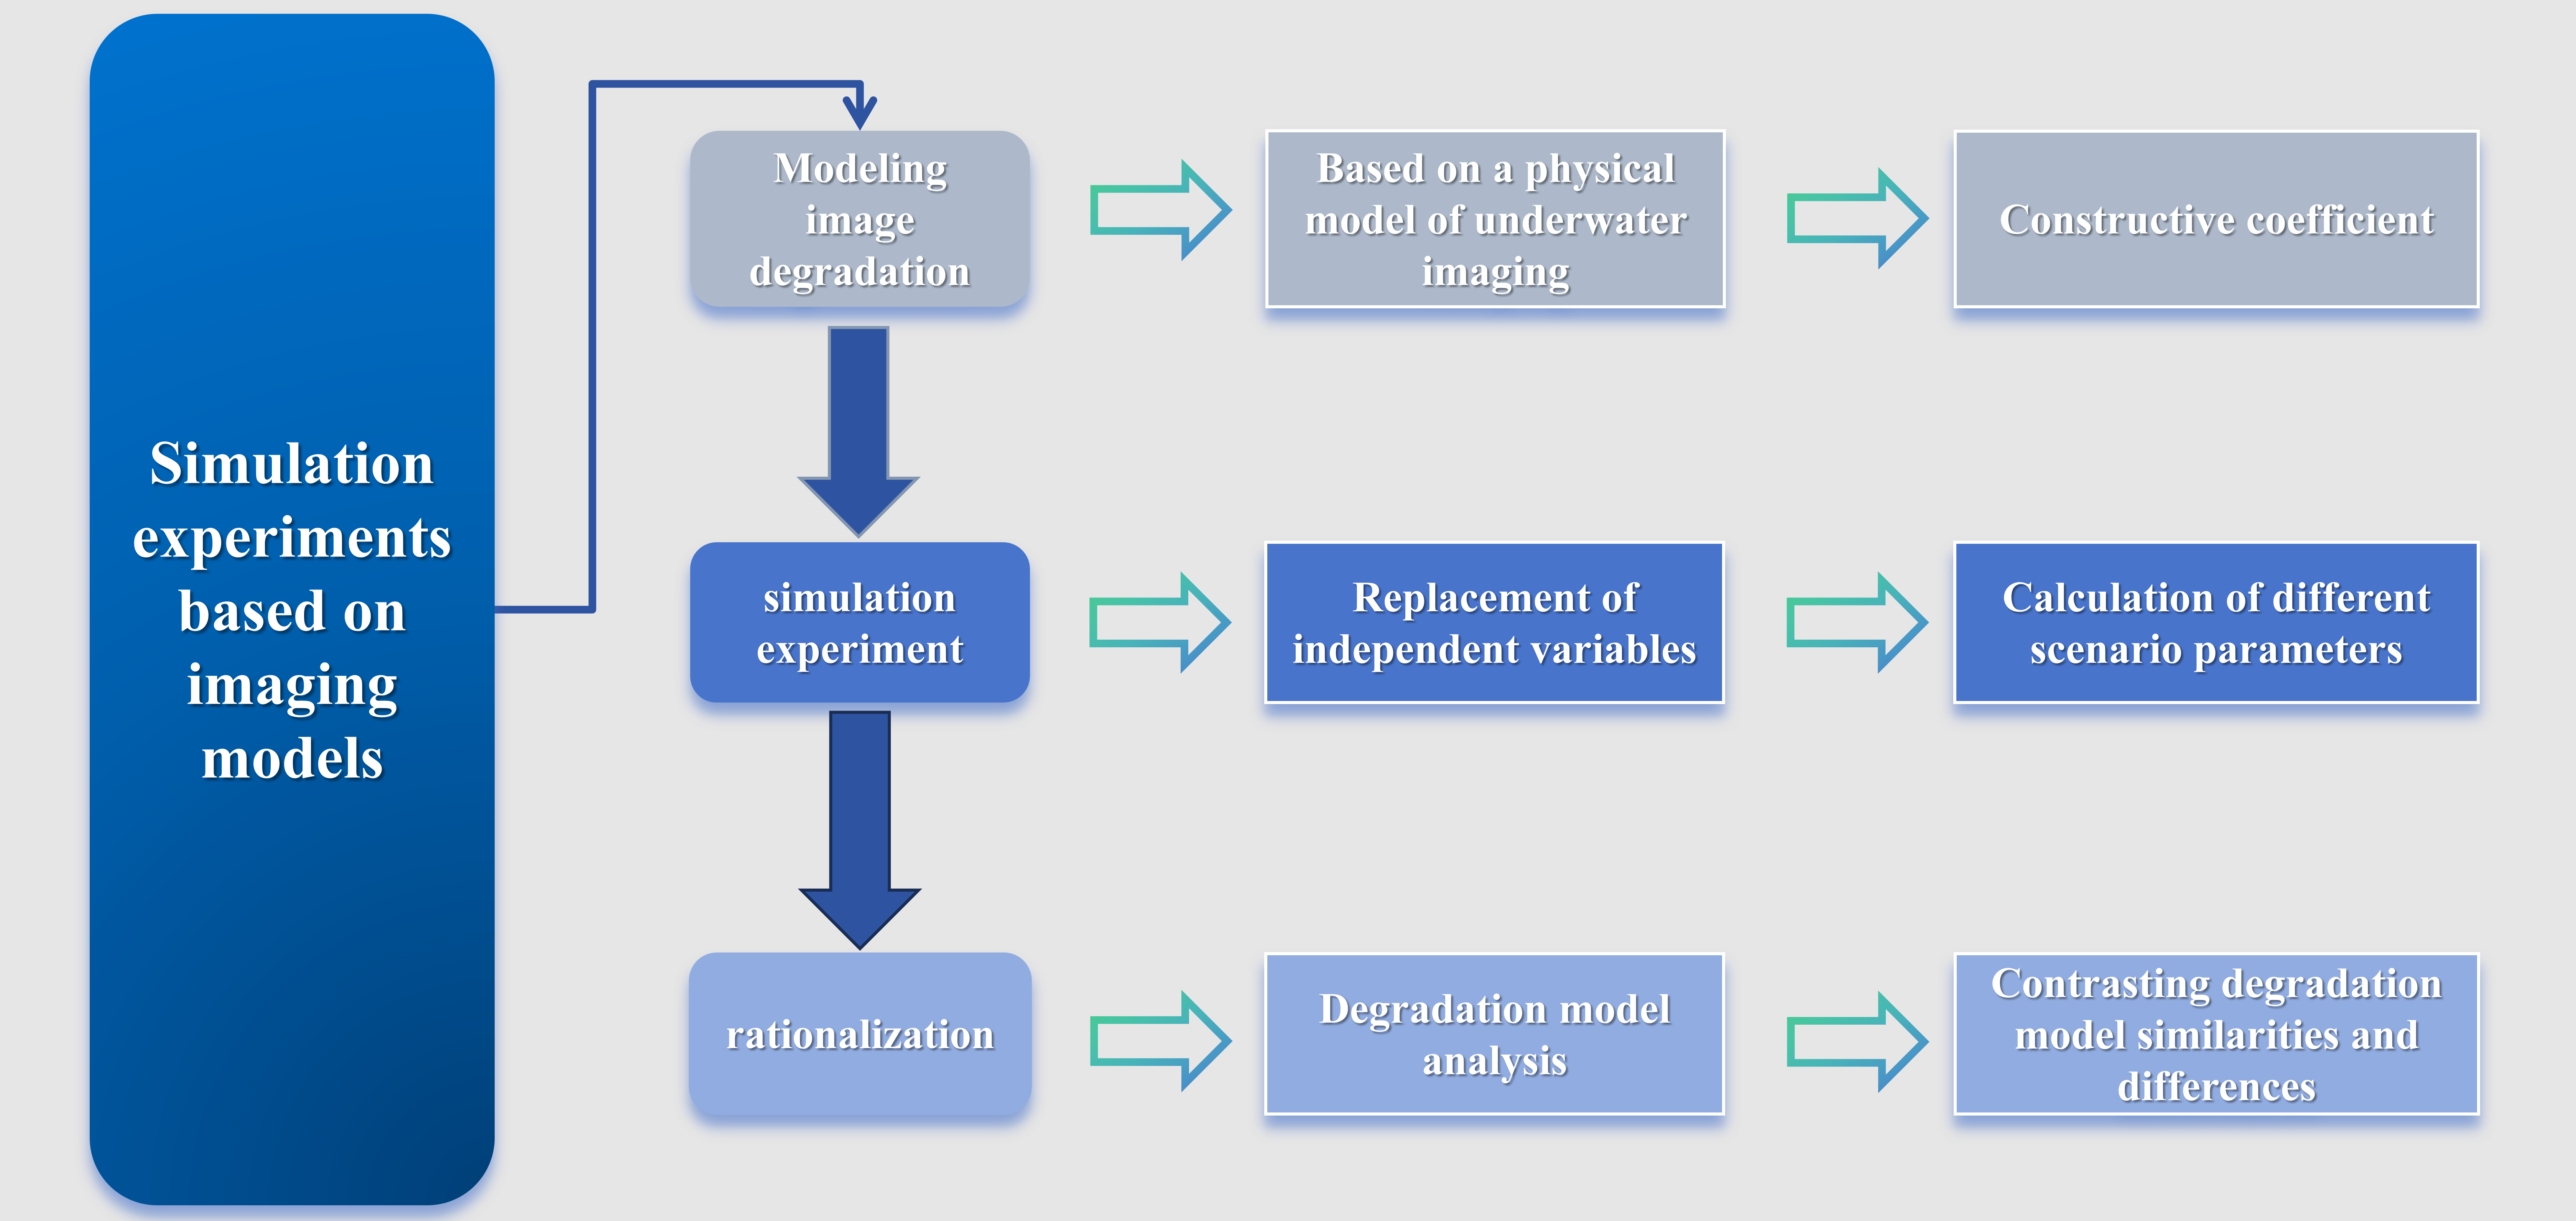
\includegraphics[width=0.75\linewidth]{figures_plus/图片1.png}
    \caption{}
    \label{fig:enter-label}
\end{figure}

In order to study the degradation characteristics of underwater images and verify the reasonableness of the related degradation models, this paper proposes a degradation modeling method based on the underwater optical transmission model proposed by Jaffe-McGlamery\textsuperscript{\cite{trucco2006self}}.

\begin{figure}[htbp]
    \centering
    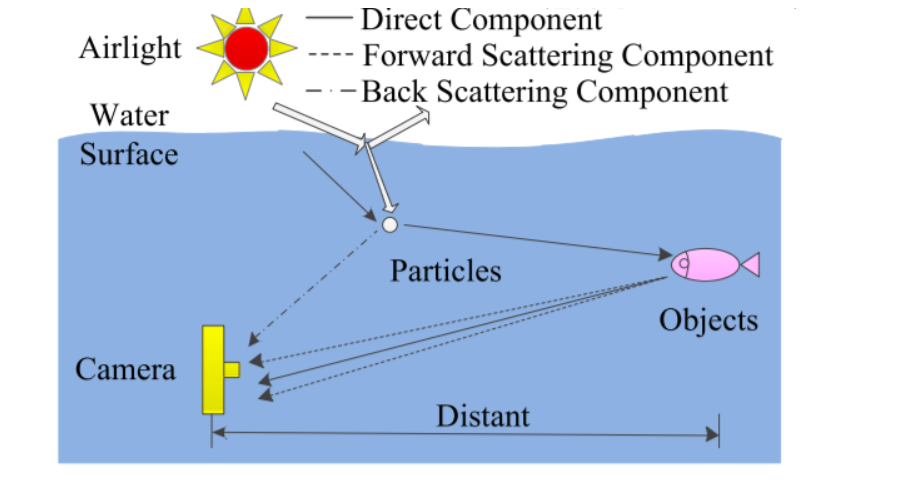
\includegraphics[width=0.75\linewidth]{figures_plus/微信图片_20241124145132.png}
    \caption{}
    \label{fig:enter-label}
\end{figure}

The model quantitatively describes degradation effects, using physical formulas to adjust core parameters (e.g., water depth d, turbidity T, background light intensity B) for generating degradation images. The degradation model is expressed as:
\[\mathrm{I}^{\mathrm{t}}(\mathrm{x})=\mathrm{J}^{\mathrm{t}}(\mathrm{x}) \cdot \mathrm{t}^{\mathrm{t}}(\mathrm{x})+\mathrm{B}_{\infty}^{t} \cdot\left(1-\mathrm{t}^{\mathrm{t}}(\mathrm{x})\right)\]

where:

\begin{itemize}[itemindent=2em]
    \item $I^t(x)$: Indicates the image signal received by the sensor after the light is attenuated by the water medium.

    \item $J^t(x)$: Indicates the direct light contribution from the target scene reflected from the target surface.

    \item $t^t(x)$:Defined as the effective percentage of light transmitted through the medium:
\end{itemize}

\[t^t(x) = \exp(-C(\lambda) \cdot r)\]

Where:

\begin{itemize}[itemindent=2em]
    \item $C(\lambda)$: the attenuation coefficient, determined by the combination of the absorption coefficient $a(\lambda)$ and the scattering coefficient $b(\lambda)$, i.e.

    \item $r$: the distance the light travels in the body of water.

    \item $B_{\infty}^{t}$:Indicates the contribution of scattered light caused by suspended solids and other media in the water body.

    \item $1 - t^t(x)$:Characterizes the degree of superimposition of background light on the degraded image and complements the transmittance $t_t(x)$.
    
\end{itemize}

\subsection{Calculation of the Optical Transmission Coefficient}

The light transmission coefficient\textsuperscript{\cite{kawaguchi1994relationship}}, denoted by $t(x)$, is a crucial parameter that characterizes the extent of light attenuation in a body of water. It quantifies the transmission effect of the reflected light, represented by $J(x)$, from the target scene. The propagation of light in a body of water is influenced by the combined effects of absorption and scattering, and its attenuation coefficient, denoted by $C(\lambda)$, is defined as:
\[C(\lambda) = a(\lambda) + b(\lambda)\]

Where:

\begin{itemize}[itemindent=2em]

    \item Absorption coefficient $a(\lambda)$ :describes the degree of light absorption by the water medium, which is calculated as:
    \[a(\lambda) = a_w(\lambda) + a_y(\lambda) + a_p(\lambda) + a_{nap}(\lambda)\]

    \item Scattering coefficient $b(\lambda)$ : describes the effect of light scattering in the water column, including the scattering of water molecules and the scattering of suspended particles, which is calculated as:
    \[b(\lambda) = b_w(\lambda) + b_{spm}(\lambda)\]

    \item The optical transmission coefficient $t(x)$ reflects the transmittance of light in the water column, and its mathematical expression is:
    \[t(x) = \exp(-C(\lambda) \cdot r)\]

    where $r$ is the depth of light propagation. Light exhibits significant differences in attenuation at different wavelengths:
        \begin{itemize}[itemindent=2em]
            \item Red light ($650 \, \text{nm}$): disappears almost completely at a depth of about $5 \, \text{m}$ due to strong absorption.  

            \item  Green light ($550 \, \text{nm}$): Significantly attenuated at a depth of about $10 \, \text{m}$.  

            \item  Blue light ($450 \, \text{nm}$): Has the strongest penetration ability, remaining high intensity at $20 \, \text{m}$ depth.  
        \end{itemize}
\end{itemize}

This wavelength dependence suggests that the optical properties of the water column have an important influence on the transmission of light of different wavelengths.

\begin{figure}[htbp]
    \centering
    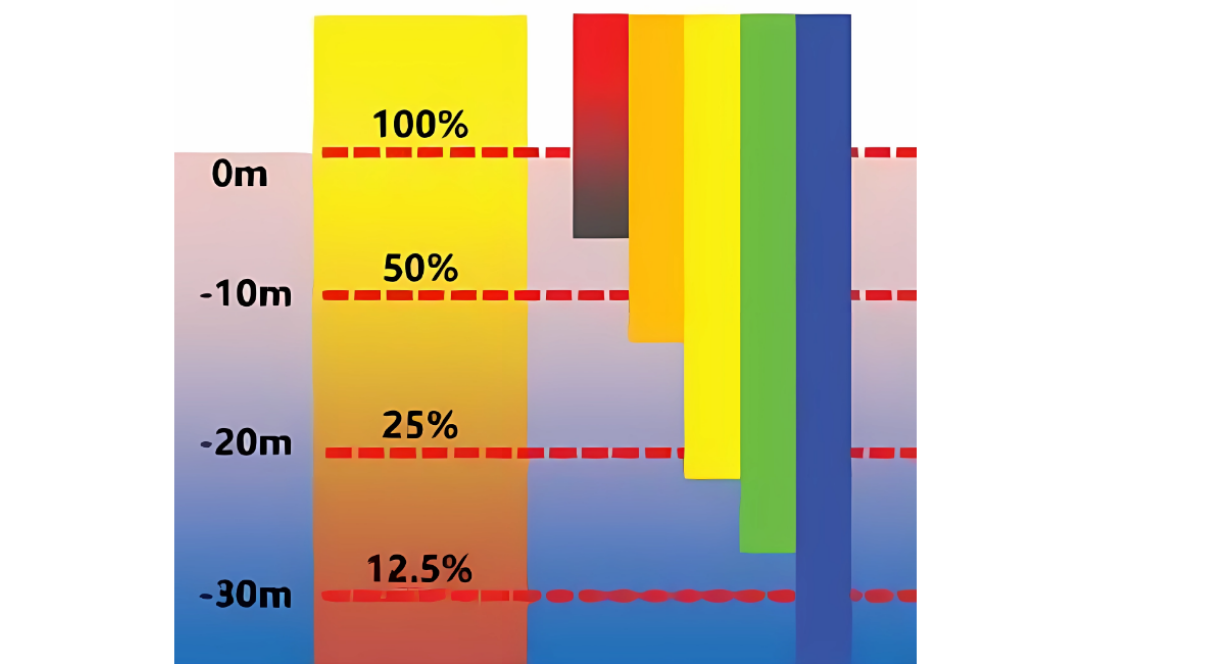
\includegraphics[width=0.75\linewidth]{figures_plus/微信图片_20241123210541.png}
    \caption{}
    \label{fig:enter-label}
\end{figure}

\subsection{Introduction of Background Light}

The incorporation of background illumination is crucial in the enhanced model to account for scattered light in underwater images. Background light refers to light entering the camera after multiple scattering events, primarily affecting brightness and contrast. Its influence is mathematically expressed as:
\[B_{\infty}^{t}\cdot (1 - t(x))\]

Where:

\begin{itemize}[itemindent=2em]
    \item  $B_{\infty}^{t}$: the ambient light intensity, which depends on the external lighting conditions. 

    \item $t(x)$: indicates the proportion of light that does not reach the target point directly, but is scattered several times. 
\end{itemize}

As t(x) decreases (due to factors like increased depth or turbidity), the proportion of background light, represented by 1 - t(x), increases. This leads to several degradation effects:

\begin{itemize}
    \item \textbf{Insufficient brightness}:  Reduced direct light transmission lowers the visibility of the target scene.
    \item \textbf{Decreased contrast}: An increased proportion of scattered light diminishes image details and sharpness.
\end{itemize}

By analyzing these degradation effects under specific conditions (e.g., with a uniform background light intensity(B = 255), the significant impact of background light on image quality is evident, offering theoretical insights for improving future enhancement algorithms.

\subsection{Simulation of Simulation Effects}

The blurring effect in underwater environments is mainly caused by forward scattering from suspended particles. To simulate this, Gaussian blurring\textsuperscript{\cite{gedraite2011investigation}} is applied based on the degradation model. The blurring is described by the formula:
\[I_{blurred}(x) = \text{GaussianBlur}(I(x), \text{kernel size})\]

Where:

\begin{itemize}[itemindent=2em]
    \item $\text{GaussianBlur}$: Gaussian blur operation for modeling scattering effects. 

    \item $\text{kernel size}$: fuzzy kernel size, used to control the degree of blurring.
\end{itemize}

By adjusting the kernel size, the blurring effect can range from slight to strong. Experimental results show that as turbidity (\(b(\lambda)\)) increases, the kernel size should also increase. Specifically:

\begin{itemize}[itemindent=2em]
    \item \textbf{Low turbidity condition}: blurring is lighter and edge details are better preserved.  

    \item \textbf{High turbidity condition}: blurring is significantly enhanced and the loss of edge details is more serious.
\end{itemize}

For high turbidity (e.g., \(b_{\text{spm}} = 0.05\), kernel size = 5), contour blurring becomes pronounced, indicating that increased turbidity severely affects image sharpness and detail. This simulation helps optimize the degradation model.

\subsection{Numerical Experiments}

\subsubsection{Design of Experiments}

In order to ascertain the validity of the underwater image degradation model, this study employs numerical simulation experiments to generate degraded images by adjusting the water depth $r$, turbidity $T$, and background light intensity $B$. The resulting images are then subjected to analysis. The specific design of the experiment is as follows:

\textbf{1.Experimental parameter settings}
 
 \begin{itemize}[itemindent=2em]

    \item  Water depth $r$: the values are $5 \, \text{m}$, $10 \, \text{m}$ and $20 \, \text{m}$, which indicate shallow water, medium depth and deep water environment, respectively. 
        
     \item Turbidity (scattering coefficient $b(\lambda)$): values of $0.01$, $0.02$ and $0.05$, corresponding to low, medium and high turbidity scenarios.  

     \item Backlight Intensity $B$: set to $50$ (for low light conditions) and $255$ (for strong light conditions).  

 \end{itemize}

 \textbf{2.Experimental steps}

\textbf{Step 1:}Read the original image $J(x)$ and separate the red, green and blue channels.

\vspace{0.5em}
\textbf{Step 2:}Calculate the transmittance $t(x)$ and calculate the absorption and scattering coefficients by wavelength:  
        \[C(\lambda) = a(\lambda) + b(\lambda)\]

\vspace{0.5em}
\textbf{Step 3:}Calculate the degraded image from the degraded model equation:
    \[I_t(x) = J_t(x) \cdot t_t(x) + B \cdot (1 - t_t(x))\]

\vspace{0.5em}
\textbf{Step 4:} Apply Gaussian blur to the degraded image to simulate the blurring effect in the underwater environment. 

\vspace{0.5em}
\textbf{Step 5:} Save the degraded image and record the following metrics: brightness, color distribution and sharpness.


 \textbf{3.Output data}

 The experimentally generated degraded images are used to analyze the following degradation characteristics:

 \begin{itemize}[itemindent=2em]
     \item Brightness: analyzed by the average pixel value of the gray scale map.  

     \item Color distortion: measured by the difference in mean values of the RGB channels.

     \item Blurriness: measured by the Laplacian (Laplace gradient) variance of the image.
 \end{itemize}

 \subsubsection{ Experimental Results and Analysis}

 In the experiment, a clear image is selected as input and 18 degraded images are generated. The properties of the generated images are analyzed and summarized as follows:

\begin{table}[!ht]
    \centering
    \setlength{\tabcolsep}{3pt} % Adjust column spacing
    \renewcommand{\arraystretch}{1.2} % Adjust row spacing
    \scriptsize % Adjust font size
    \begin{tabular}{cccccccc}
        \toprule
        \makecell{\textbf{Water depth} \\ \boldmath{$d$}} & 
        \makecell{\textbf{Turbidity} \\ \boldmath{$T$}} & 
        \makecell{\textbf{Background} \\ \textbf{light} \boldmath{$B$}} & 
        \makecell{\textbf{Luminance} \\ \textbf{mean}} & 
        \makecell{\textbf{Red light} \\ \textbf{mean}} & 
        \makecell{\textbf{Green light} \\ \textbf{mean}} & 
        \makecell{\textbf{Blue light} \\ \textbf{mean}} & 
        \makecell{\textbf{Sharpness}} \\ 
        \midrule
        5m & 10 & 50 & 125.6 & 85.2 & 95.6  & 120.4  & 10.2  \\ 
        5m & 10 & 225 & 160.8 & 100.4 & 110.5  & 140.3  & 10.2  \\ 
        5m & 20 & 50 & 115.3 & 78.3 & 88.7  & 110.5  & 9.4  \\ 
        5m & 20 & 225 & 144.9 & 93.2 & 103.4  & 130.7  & 9.4  \\ 
        5m & 50 & 50 & 110.7 & 70.1 & 85.3  & 115.7 & 8.3  \\ 
        5m & 50 & 225 & 140.4 & 85.3 & 98.2  & 135.4  & 8.3  \\ 
        10m & 10 & 50 & 105.3 & 65.4 & 80.6  & 110.2  & 8.7  \\ 
        10m & 10 & 225 & 135.2 & 80.3 & 95.2  & 130.5 & 8.7  \\ 
        10m & 20 & 50 & 90.2 & 50.1 & 65.2  & 95.4  & 7.6  \\ 
        10m & 20 & 225 & 120.6 & 70.8 & 80.4  & 115.2  & 7.6  \\ 
        10m & 50 & 50 & 84.7 & 40.1 & 55.6  & 90.2  & 6.7  \\ 
        10m & 50 & 225 & 115.3 & 60.7 & 70.4  & 110.1  & 6.7  \\ 
        20m & 10 & 50 & 85.2 & 40.5 & 55.3  & 90.6  & 7.4  \\ 
        20m & 10 & 225 & 115.3 & 60.2 & 75.1 & 110.8  & 7.4  \\ 
        20m & 20 & 50 & 75.6 & 30.3 & 45.2  & 85.2  & 6.2  \\ 
        20m & 20 & 225 & 105.2 & 50.3 & 65.6  & 105.7 & 6.2  \\ 
        20m & 50 & 50 & 70.3 & 20.4 & 35.6  & 80.2  & 5.4  \\ 
        20m & 50 & 225 & 100.5 & 40.6 & 50.8  & 100.3  & 5.4  \\ 
        \bottomrule
    \end{tabular}
\end{table}



By observing the experimental results, the following analytical conclusions can be drawn:

\textbf{1.} In the underwater environment, the change of image brightness is closely related to the water depth $d$ and turbidity $T$. The experimental results show that:

\begin{itemize}[itemindent=2em]
    \item As a consequence of the increase in both $d$ and $T$, the attenuation effect of light is significantly enhanced, resulting in a significant decrease in the average value of image brightness.

    \item Under the high turbidity condition in deep water ($d = 20 \, \text{m}, \, T = 0.05$), the image brightness is only $70.3$, which shows an obvious overall darkening effect.

    \item An augmentation of the background light intensity, designated as $B$, can enhance the brightness to a certain degree. To illustrate, when $B = 255$, the brightness is augmented by approximately $30\%$ in comparison to the low light condition, which effectively addresses the issue of insufficient brightness.
\end{itemize}

\textbf{2.} Color distortion is another significant feature of underwater image degradation, especially in the absorption difference of different wavelengths of light:

\begin{itemize}[itemindent=2em]
    \item \textbf{Red light} has the most significant absorption, which gradually disappears with the increase of water depth and turbidity. In deep water with high turbidity, the average value of red light is only $20.1$, which is almost completely absorbed.

    \item \textbf{Blue light,} being the most penetrating, dominates the light intensity in all scenes, and the image as a whole shows a distinct blue-green hue.
\end{itemize}

These variations are highly consistent with the underwater optical properties, verifying the reasonableness of the degradation model.

\begin{figure}[htbp]
    \centering
    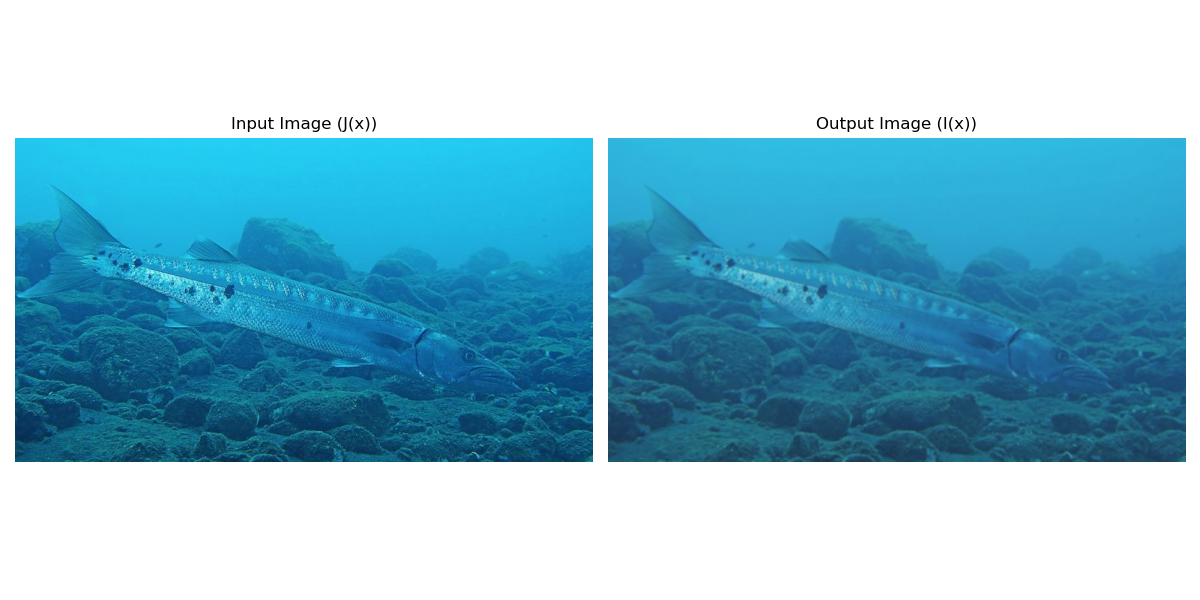
\includegraphics[width=0.75\linewidth]{figures_plus/061c1e0fcc91825b840be17f18c090a.png}
    \caption{}
    \label{fig:enter-label}
\end{figure}

The degree of ambiguity is mainly determined by the turbidity in the water column. The experimental results show that:

\begin{itemize}[itemindent=2em]
    \item \textbf{Blurring:}The blurring effect (measured by Laplacian gradient variance) increases with turbidity, with sharpness dropping significantly in high turbidity conditions (T = 0.05), where edge details are almost lost and sharpness reaches 5.4.

    \item \textbf{Background light intensity:} Increasing background light (B) improves brightness but has limited impact on blurring and edge sharpness.

\end{itemize}

Key conclusions:

\begin{itemize}[itemindent=2em]
    \item \textbf{Insufficient brightness:} Water depth and turbidity reduce image brightness, particularly in deep and high turbidity conditions. Increasing background light intensity (B) can help improve brightness.

    \item \textbf{Color distortion:} Red light is most absorbed at shallow depths, disappearing as depth increases, leading to a blue-green hue, which aligns with observed underwater optical properties and supports the degradation model.

    \item \textbf{Blurring effect:} The degree of blurring is primarily attributable to turbidity.  In circumstances characterised by elevated turbidity levels, the image clarity is markedly diminished, as evidenced by the loss of edge details and the blurring of contours.
\end{itemize}


%%%%%%%%%%%%%%%%%%%%%%%%%%%%%%%%%%%%%%%%%%%%%%%%%%%%%%%%%%%%%
\newpage
\section{Establishment and Solution of the Model of Question 3}

In the field of underwater image processing, enhancement methods are employed with the objective of restoring and improving the quality of degraded images. This is achieved by addressing issues such as low light, color distortion, and blurring. For a specific type of degradation, such as low light, color shift, or blur, targeted enhancement methods can be designed to enhance the visual quality and information retention of the image.
\[I(x) = J(x) \cdot t(x) + B \cdot (1 - t(x))\]

Where:

\begin{itemize}[itemindent=2em]
    \item $I(x)$ is the observed degraded image;  

    \item $J(x)$ is the reflected light image of the target scene;  

    \item $t(x)$ denotes the transmittance, which reflects the degree of light attenuation in water;  

    \item $B$ is the background light intensity, which is used to simulate the effect of multiple scattered light on the image.
\end{itemize}

\begin{figure}[htbp]
    \centering
    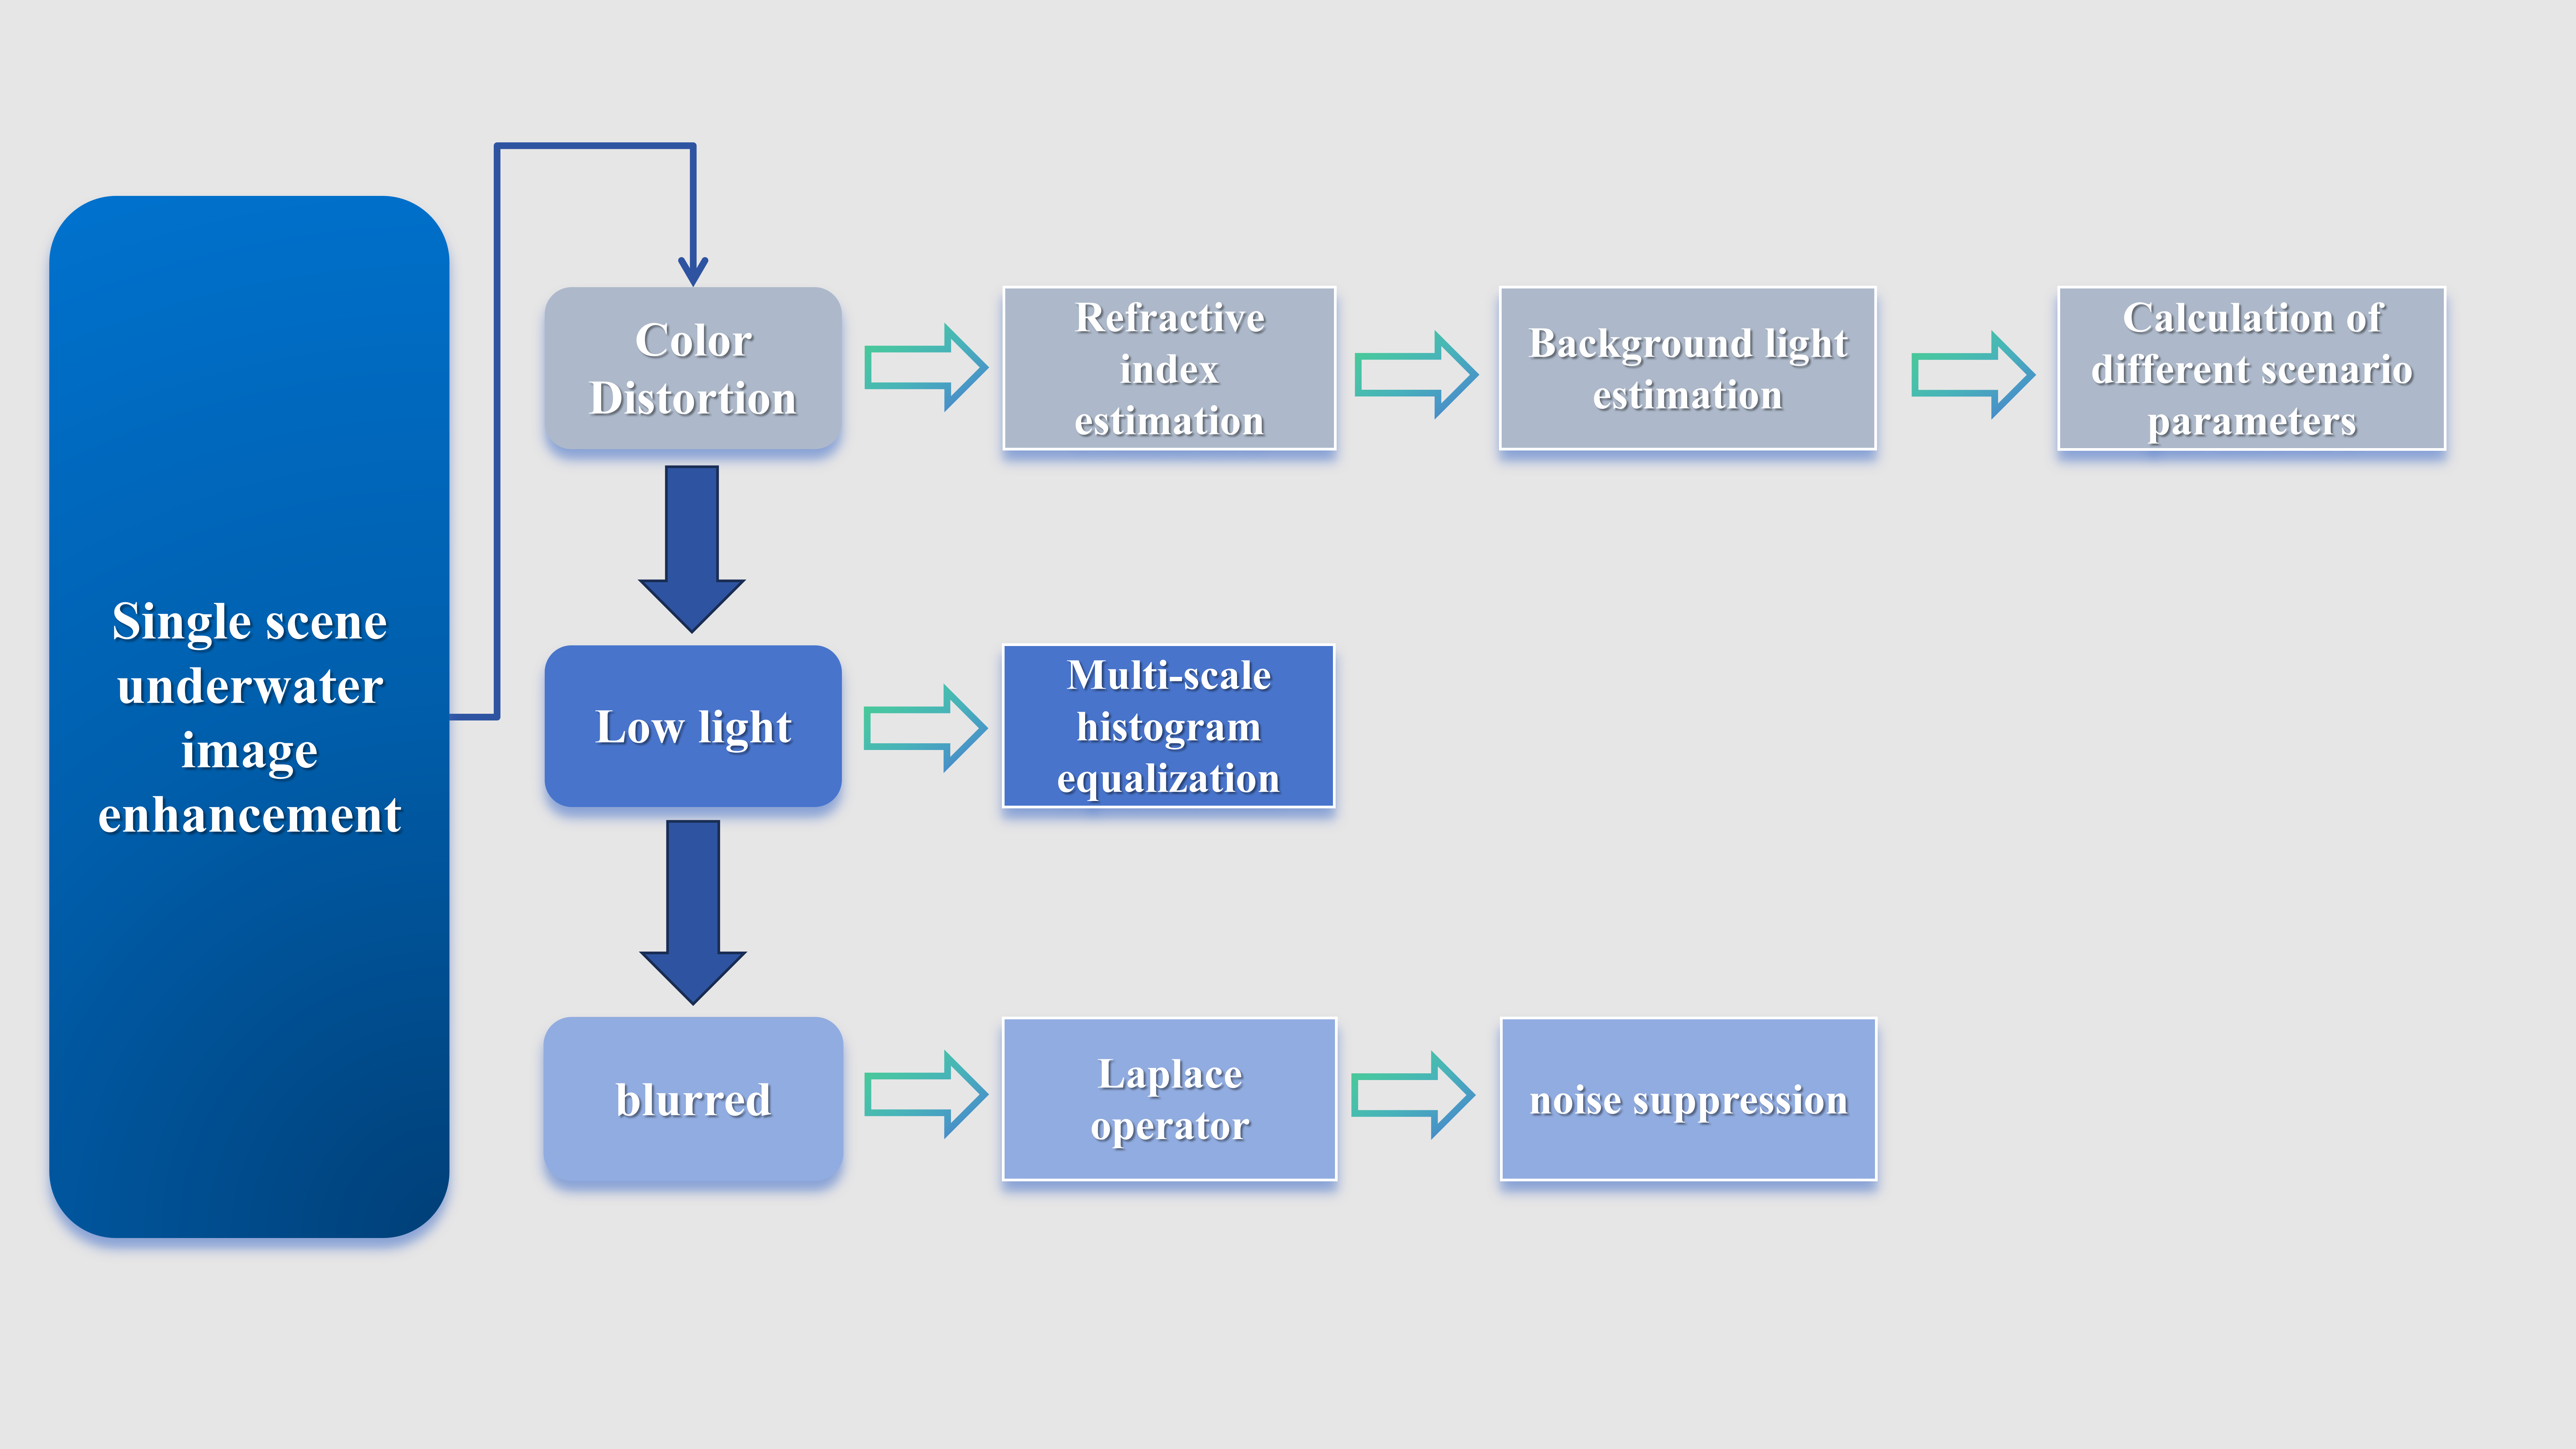
\includegraphics[width=0.75\linewidth]{figures_plus/微信图片_20241124120242.png}
    \caption{}
    \label{fig:enter-label}
\end{figure}

\subsection{Enhancement Methods for Low Light }

Low-light images in underwater environments are caused by light absorption and scattering, leading to reduced brightness, contrast, and loss of details.

This paper proposes a Multi-Scale Histogram Equalization (MSHE)\textsuperscript{\cite{brown2005multi}} method to enhance both brightness and contrast. MSHE divides the image into subregions, adjusts pixel values based on local histograms, and combines the results using multi-scale fusion to improve image quality while preserving details.

\textbf{Steps for multi-scale histogram equalization}

\textbf{Step 1:} Image Chunking: Divide the input image into local subregions, each consisting of a block of pixels (e.g., 8×8 or 16×16). Each subregion is analyzed independently for luminance distribution.

\vspace{0.5em}
\textbf{Step 2:}Local Histogram Calculation: For each subregion, calculate a luminance histogram to obtain the region’s luminance distribution. Based on the histogram, an equalization mapping function is generated to adjust the luminance distribution to a target range.

\vspace{0.5em}
\textbf{Step 3:}Local Enhancement: Apply the equalization mapping function to each subregion to enhance the brightness, contrast, and local detail of the image.

\vspace{0.5em}
\textbf{Step 4:}Multi-Scale Fusion: Perform equalization at various scales, starting from the smallest regions to the largest. The enhanced results are then combined to create the final image, balancing the enhancement of local details with the overall visual effect.         


The fusion formula is as follows:
\[I_{i}(x, y) = \sum_{i=1}^{N} w_i I_i(x, y)\]

Where:

\begin{itemize}[itemindent=2em]
    \item $I_i(x, y)$ denotes the enhanced image at the $i$th scale;

    \item $w_i$ denotes the weight at the $i$th scale satisfying $\sum_{i=1}^{N} w_i = 1$.
\end{itemize}

\subsection{An Enhancement Method for Color Distortion}

Color distortion in underwater images arises due to the differential absorption and scattering of light. Red light is strongly absorbed, while blue light penetrates the deepest, leading to a blue-green color cast. This distortion hinders object recognition and analysis. This paper proposes a method based on wavelength compensation and contrast correction to restore the true color of the image.

\subsubsection{The Principle of Wavelength Compensation}

The goal is to recover lost color information due to light attenuation. The image degradation model is:
\[I(x) = J(x) \cdot t(x) + B \cdot (1 - t(x))\]

In this model, $I(x)$ represents the degraded image, $J(x)$ represents the clear image without degradation, $t(x)$ represents the transmittance of light in water, and $B$ represents the background light intensity. The degradation model describes the contribution of directly reflected light (related to $J(x) \cdot t(x)$) and background scattered light (related to $B \cdot (1 - t(x))$) in the image.

\subsubsection{Estimation of the Refractive Index}

The transmittance, denoted by $t(x)$, is a measure of the proportion of incident light that can be transmitted through a body of water after undergoing absorption and scattering processes. It is calculated as follows:
\[t(x) = \exp(-C(\lambda) \cdot r)\]

In this context, the wavelength-dependent attenuation coefficient, denoted by $C(\lambda),$ is a function of the wavelength, whereas the depth of propagation of light, represented by $r,$ is a function of the depth. As direct measurement of $t(x)$ is challenging in practical applications, this paper employs the dark channel assumption to estimate the transmittance. The dark channel theory posits that in a clear image, the majority of non-sky regions exhibit at least one color channel with a value approaching zero. Consequently, the transmittance can be estimated by the following equation:
\[t(x) = 1 - w \cdot \min_{y \in \Omega(x)} \left( \min_c I_c(y) \right)\]

In this method, the adjustment factor ($w$, typically taken as 0.95), the neighborhood window of pixel $x$ ($\Omega(x)$), and the background light intensity ($Bc$) are used to estimate the transmittance of different regions in the image. This provides a basis for recovering the true color.

\subsubsection{Estimation of Background Light}

The background light, designated as $B$, represents the primary source of scattered light in a body of water. Its intensity is influenced by a combination of ambient light and the oiliness of the water body. In images exhibiting color distortion, the background light is typically estimated based on the brightness of the image's brightest areas. This paper presents a methodology for estimating the background light intensity, which involves:
\[B_c = \max I_c(x), \quad x \in \Omega(I)\]

\subsubsection{Contrast Correction}

After wavelength compensation and color restoration, the image may still suffer from insufficient contrast, especially in highly turbid waters. To address this, this paper utilizes the Contrast-Limited Adaptive Histogram Equalization (CLAHE)\textsuperscript{\cite{reza2004realization}} technique to enhance the contrast of the restored image. The process is as follows:

\begin{itemize}
    \item Convert the image from RGB space to LAB color space;

    \item apply CLAHE to the luminance channel $L$ to avoid over-enhancement by limiting the contrast. 3;

    \item merge the enhanced $L$ channel with the original $A$ and $B$ channels to restore the image to RGB.
\end{itemize}

This contrast correction significantly improves the visual quality of the image, enhancing color richness and making details more prominent.

\subsection{Enhancement Methods for Blurring}

The blurring phenomenon in underwater images is primarily caused by the scattering effect of light, particularly multiple scattering by suspended particles in the water. This results in blurred edges and loss of detail in the image. 

Additionally, high water turbidity exacerbates the blurring, making it difficult to recognize target objects. This blur not only affects image clarity but also presents significant challenges for underwater target recognition, navigation, and measurement.

To address this issue, this paper proposes a methodology based on Laplacian sharpening. This approach enhances image clarity by emphasizing the details at the edges, while effectively avoiding the noise amplification issues often encountered with traditional sharpening algorithms.

\subsubsection{Fuzzy Degradation}

Fuzzy degradation can usually be described by a convolution operation with the following formula:
\[I_{\text{blurred}}(x, y) = I_{\text{original}}(x, y) * h(x, y) + n(x, y)\]

Where:

\begin{itemize}[itemindent=2em]
    \item $I_{\text{blurred}}(x, y)$ is the degraded blurred image;

    \item $I_{\text{original}}(x, y)$ is the original clear image;

    \item $h(x, y)$ is the blurring kernel (PSF, point spread function), which describes the blurring effect caused by light scattering;

    \item $n(x, y)$ is the image noise.
\end{itemize}

In order to eliminate the blurring effect, it is typically necessary to estimate and deconvolve the blurring kernel, $h(x,y)$. However, since the actual blurring kernel is challenging to estimate with precision, this paper employs a sharpening method based on the Laplacian operator to enhance the details of the blurred image directly.

\subsubsection{Laplacian Operator}

The Laplacian operator is a second-order derivative operator that is utilized to detect edge information in an image. Laplacian sharpening serves to enhance the edge contrast and details by adding the image with its Laplacian operator filtering result. Its mathematical formula is as follows:
\[I_{\text{sharp}}(x, y) = I_{\text{blurred}}(x, y) + \lambda \cdot \Delta I(x, y)\]

Where:

\begin{itemize}[itemindent=2em]
    \item $I_{\text{sharp}}(x, y)$ is the enhanced sharp image;

    \item $\Delta I(x, y) = \nabla^2 I(x, y)$ is the Laplace operator of the image;

    \item $\lambda$ is the sharpening intensity factor, which controls the magnitude of the detail enhancement.
\end{itemize}

The Laplace operator can be computed using the following discrete convolution kernel:
\[\begin{bmatrix}
0 & 1 & 0 \\
1 & -4 & 1 \\
0 & 1 & 0
\end{bmatrix}\]

The formula primarily serves to enhance the high-frequency information (such as edges and details) within the image, while simultaneously reducing the blurring phenomenon caused by scattering.

\subsubsection{Noise Suppression}

In images with a low signal-to-noise ratio, the addition of noise may be confounded with the presence of edges, and direct sharpening may result in the amplification of noise. To circumvent this issue, this paper employs a Gaussian blurring technique prior to sharpening, thereby mitigating the effects of noise. The specific methodology is outlined below:

\textbf{Step 1:} Perform Gaussian filtering on the blurred image $I_{\text{blurred}}(x, y)$:
\[I_{\text{smoothed}}(x, y) = I_{\text{blurred}}(x, y) * G(x, y)\]

where $G(x, y)$ is a Gaussian kernel for noise suppression.

\vspace{0.5em}
\textbf{Step 2:}Apply the Laplace sharpening formula on top of the smoothed image so as to avoid noise enhancement.

By this method, the negative impact of noise on image quality can be effectively suppressed while enhancing the image details.


%%%%%%%%%%%%%%%%%%%%%%%%%%%%%%%%%%%%%%%%%%%%%%%%%%%%%%%%%%%%%
\newpage
\section{Establishment and Solution of the Model of Question 4}

To address Question four, we propose an underwater image enhancement model for complex scenes, based on the fusion principle. This method uses only the degraded image to generate inputs and weighting metrics. To mitigate the effects of the underwater medium, two inputs are defined: a color-corrected version and a contrast-enhanced version of the original image. Additionally, four weighting maps are designed to address reduced visibility of distant objects due to scattering and absorption.


Our approach is a single-image enhancement method that requires no special hardware and does not rely on a priori knowledge of underwater conditions or scene structure. The enhanced images and videos show reduced noise, improved exposure in dark areas, higher overall contrast, and optimized fine details and edges, effectively handling degraded images in underwater scenes. low-light, and blurred scenes.

\begin{figure}[htbp]
    \centering
    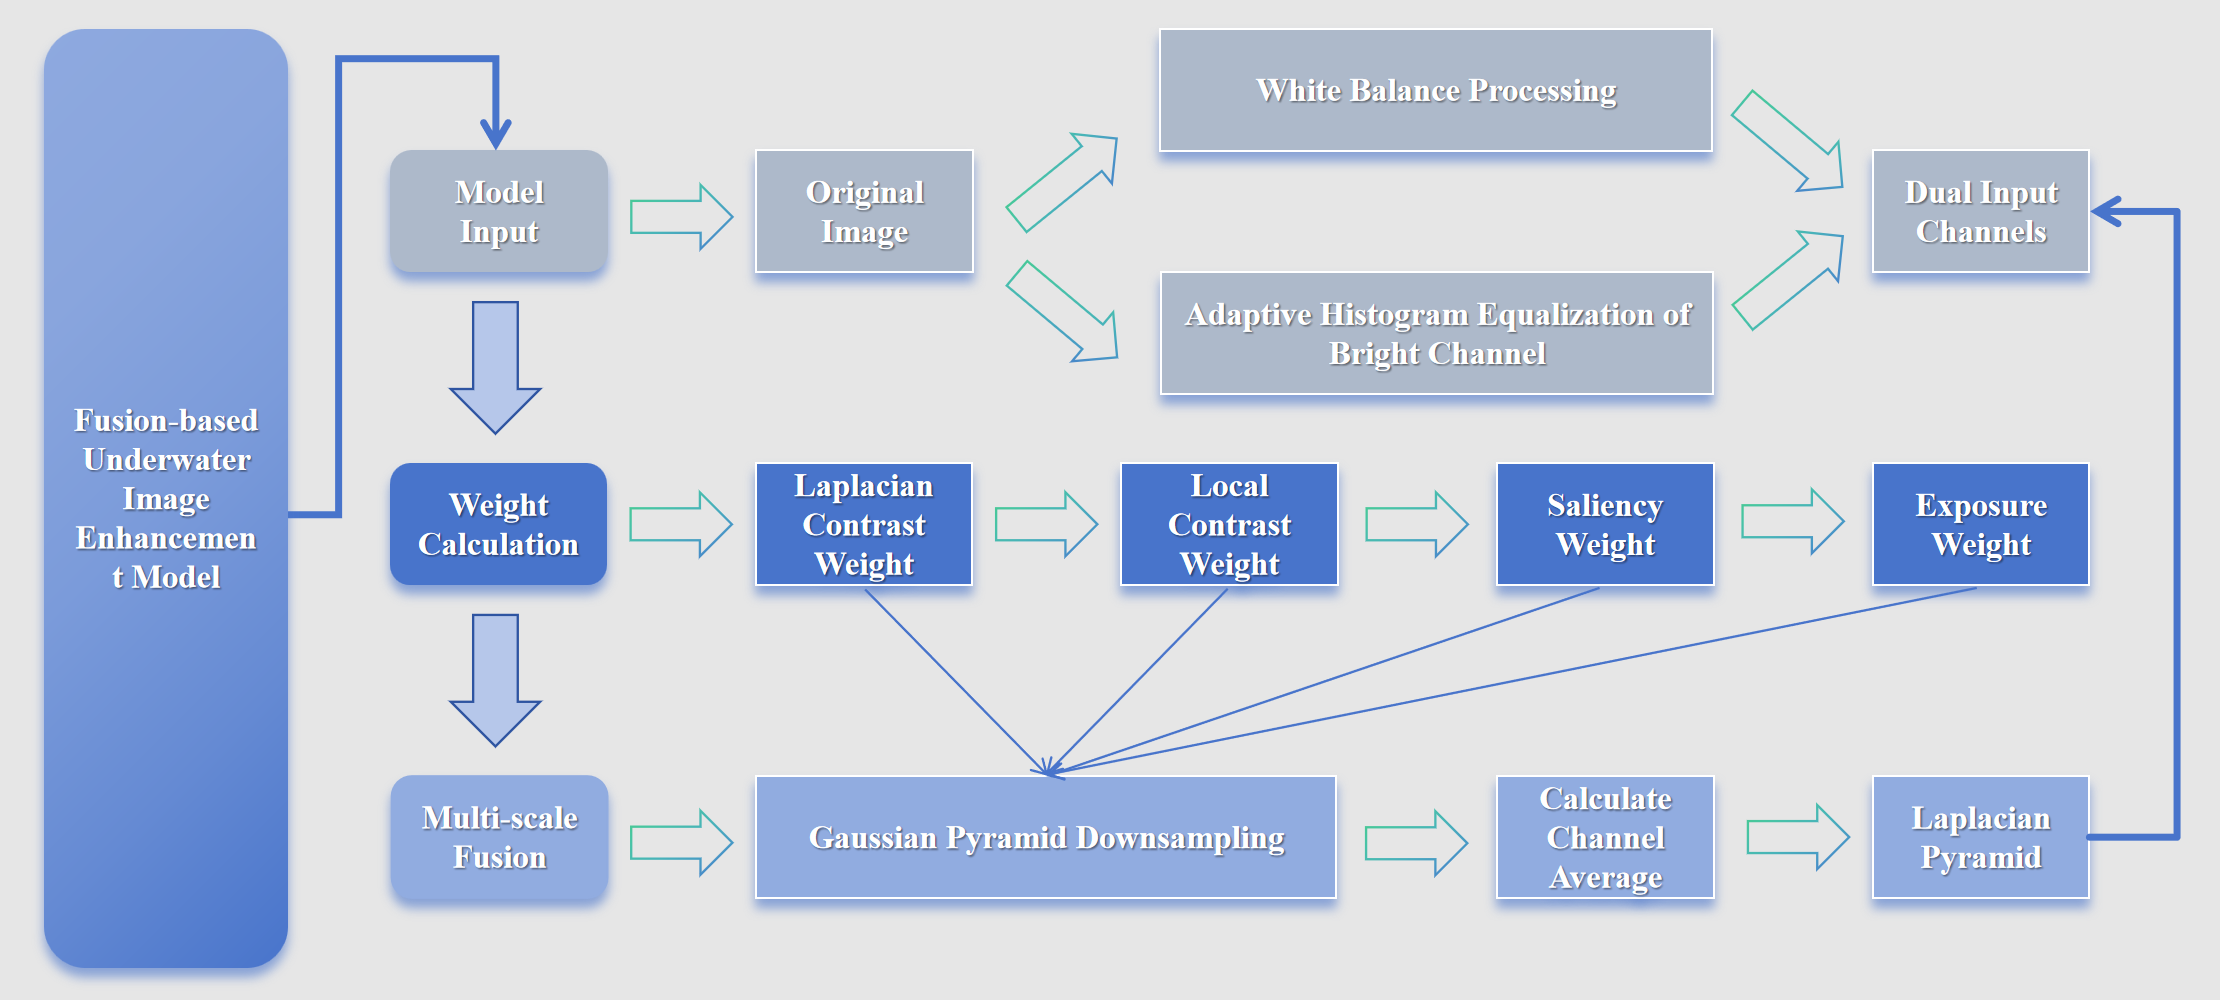
\includegraphics[width=0.75\linewidth]{figures_plus/流程图4.png}
    \caption{}
    \label{fig:enter-label}
\end{figure}


\subsection{ Input of the Fusion Process}

For underwater image fusion, we aim to retain key features and improve visual quality. Our method uses two inputs derived from the original degraded image: a color-corrected version and a contrast-enhanced image after noise reduction.

\subsubsection{White Balancing of the Inputs}

The first input is obtained through white balancing to remove color casts from different light sources. In deep water, white balance can be difficult due to light absorption, so we use the illumination value (µI), calculated from the average luminance (µref) of the scene, adjusted by parameter $\lambda$:
\[\mu_{I} = 0.5 + \lambda_{\mu_{ref}}\]

The value of λ is determined based on the color histogram distribution. A value of λ = 0.2 typically provides good results for most underwater images, improving color balance and creating a natural look. However, white balance alone cannot address visibility issues, so we use a second input for contrast enhancement.

\subsubsection{Image Denosing of the Inputs}

Due to impurities in the underwater environment and special lighting conditions, underwater images are often accompanied by a high level of noise. Methods such as median filtering, anisotropic diffusion, and bilateral filtering can be used to remove the noise while preserving the edges of the image. For video, the need to consider both spatial and temporal coherence makes the task even more challenging. The bilateral filter\textsuperscript{\cite{elad2002origin}} is a non-iterative, edge-preserving smoothing filter commonly used in tone mapping and anti-aliasing scenarios. Its formula is:
\[J_{s}=\frac{1}{k(s)} \sum_{p \in \Omega} f\left(p-s, \sigma_{f}\right) g\left(D(p, s), \sigma_{g}\right) I_{p}\]

Where:

\begin{itemize}[itemindent=2em]
    \item $D(p,s)=I_{p}- I_{s}$ denotes the pixel intensity difference, 

    \item k(s) is the normalization factor.
\end{itemize}

However, bilateral filtering does not guarantee temporal consistency. For dynamic scenes, we apply a temporal bilateral filtering strategy to white-balanced images to reduce noise and smooth frames while maintaining temporal consistency, following the method of Bennett et al. For further optimization, the sum of squared differences (SSD) of the spatial neighborhood $\psi$ is computed and Eq:
\[\psi D(p, s)=\sum_{x, y \in \Psi} \Gamma(x, y)\left(I_{p}-I_{s}\right)^{2}\]

Larger neighborhood sizes (e.g., 3 × 3 or 5 × 5) help reduce the impact of single-pixel noise.

In the fusion framework, the second input is based on the noise-reduced and color-corrected image, and contrast is enhanced using Local Adaptive Histogram Equalization (CLAHE), which is highly automated, less distorted, and expands the contrast of the region of interest to maximize contrast between neighboring structures. For further enhancement, more sophisticated methods such as Multi-Scale Retinex (MSR) can be used. Ultimately, this input is used to mitigate the degradation caused by volume scatter and optimize the contrast level of the image.

\subsection{Weights of the Fusion Process}

Weighting is crucial in underwater image enhancement, aiming to assign appropriate weights to different regions based on the expected appearance of the restored image, ensuring a natural and detailed fusion result. Since image restoration is closely tied to color appearance, simple per-pixel fusion is inadequate for integrating key features, contrast, and exposure information, potentially introducing artifacts. 

Thus, four weights are designed: Laplace contrast weight, local contrast weight, saliency weight, and exposure weight. These weights emphasize key features, balance global and local contrast, enhance salient areas, and preserve natural luminance distribution, addressing the three main degradation issues of underwater images.

\vspace{0.5em}
\textbf{1.Laplace contrast weighting ($W_{L}$)}

The Laplace contrast weighting measures the global contrast by applying a Laplace filter to the luminance channel of the input image and calculating the absolute value of the filter result. This weighting can effectively emphasize the edge and strand details in the image to make the fusion result clearer. The formula is:
\[W_2(x, y) = \left| \nabla^2 I_k(x, y) \right|\]

Where:

\begin{itemize}[itemindent=2em]

    \item $\nabla^2 I_k(x, y)$ denotes the Laplace filter value of the luminance channel at pixel (x, y).
    
\end{itemize}

\vspace{0.5em}
\textbf{2.Weighting of local contrast ($W_{LC}$)}

The Local Contrast weight enhances the local contrast effect by measuring the difference between each pixel value and its neighborhood average. It focuses on highlighting details in the highlights and shadows of the image, making the layers between neighboring structures more distinct. The formula is:
\[W_{LC}(x, y) = \left| I_k(x, y) - I_k^{Wh_c}(x, y) \right|\]

\vspace{0.5em}
\textbf{3.Significance weights ($W_{s}$)}

The saliency weight is used to highlight the target areas that are not easily noticed in the underwater scene, and to enhance the presence of the target objects in the fused image by detecting the saliency characteristics of the image. It is inspired by the “center-surround contrast” mechanism in biology, and is calculated as follows:
\[W_{s}(x, y) = \left| I_{k}(x, y) - I_{k}^{avg} \right| \]

where $I_{k}^{avg}$ is the global average brightness value of the image, $\left| I_{k}(x, y) - I_{k}^{avg} \right|$ indicates the degree of contrast between the pixel and the global average brightness. The significance weights prioritize the emphasis on high contrast regions, highlighting the difference between the background and the target.

\vspace{0.5em}
\textbf{4.Exposure Weight ($W_{E}$)}

Exposure weights are used to measure the exposure level of a pixel, protecting the middle brightness area so that the fusion result is neither overexposed nor too dark. It calculates the exposure level of a pixel using a Gaussian distribution model with the following formula:
\[W_E(x, y) = \exp\left(-\frac{(I_k(x, y) - 0.5)^2}{2\sigma^2}\right)\]

\vspace{0.5em}
\textbf{5.Weight Normalization}

To ensure that the weights are balanced, all the weights are finally normalized by Eq:
\[\bar{W}^k(x, y) = \frac{W^k(x, y)}{\sum_{k=1}^{K} W^k(x, y)}\]

\subsection{Multi-scale Fusion Process}

The enhanced image R(x, y) is computed by fusing the defined inputs with the weights of each pixel position, which is given by Eq:
\[R(x, y) = \sum_{k=1}^{K} \bar{W}^k(x, y) I_k(x, y)\]

Where:

\begin{itemize}[itemindent=2em]
    \item $I_{k}$ denotes the kth input (in this paper k = 2) ,

    \item ${W}^k$ is the normalized weight map.
\end{itemize}

The normalization process ensures that the weight of each pixel position is summed to 1, thus maintaining the proportionality of the different weights during the fusion process. However, the direct use of this parsimonious fusion method may introduce undesired vignetting or artifacts.However, the direct use of this plain fusion method may introduce undesired halos or artifacts.

To address this issue, we propose a fusion strategy based on multi-scale Laplacian pyramid decomposition. This method processes image characteristics at multiple scales, effectively reducing artifacts, enhancing details, and preserving the overall naturalness of the image. The specific process is as follows:

\vspace{0.5em}
\textbf{1.Laplace Decomposition}

Each input image is first decomposed into multi-scale quasi-bandpass versions by Laplace pyramid decomposition. Specifically, the input image is first convolved with a Gaussian kernel to generate a low-pass filtered version, and then the difference between the original image and the low-pass filtered image is calculated. By iterating layer by layer in this way, the detailed features at different frequencies are extracted to form the Laplacian pyramid representation.

\begin{figure}[htbp]
    \centering
    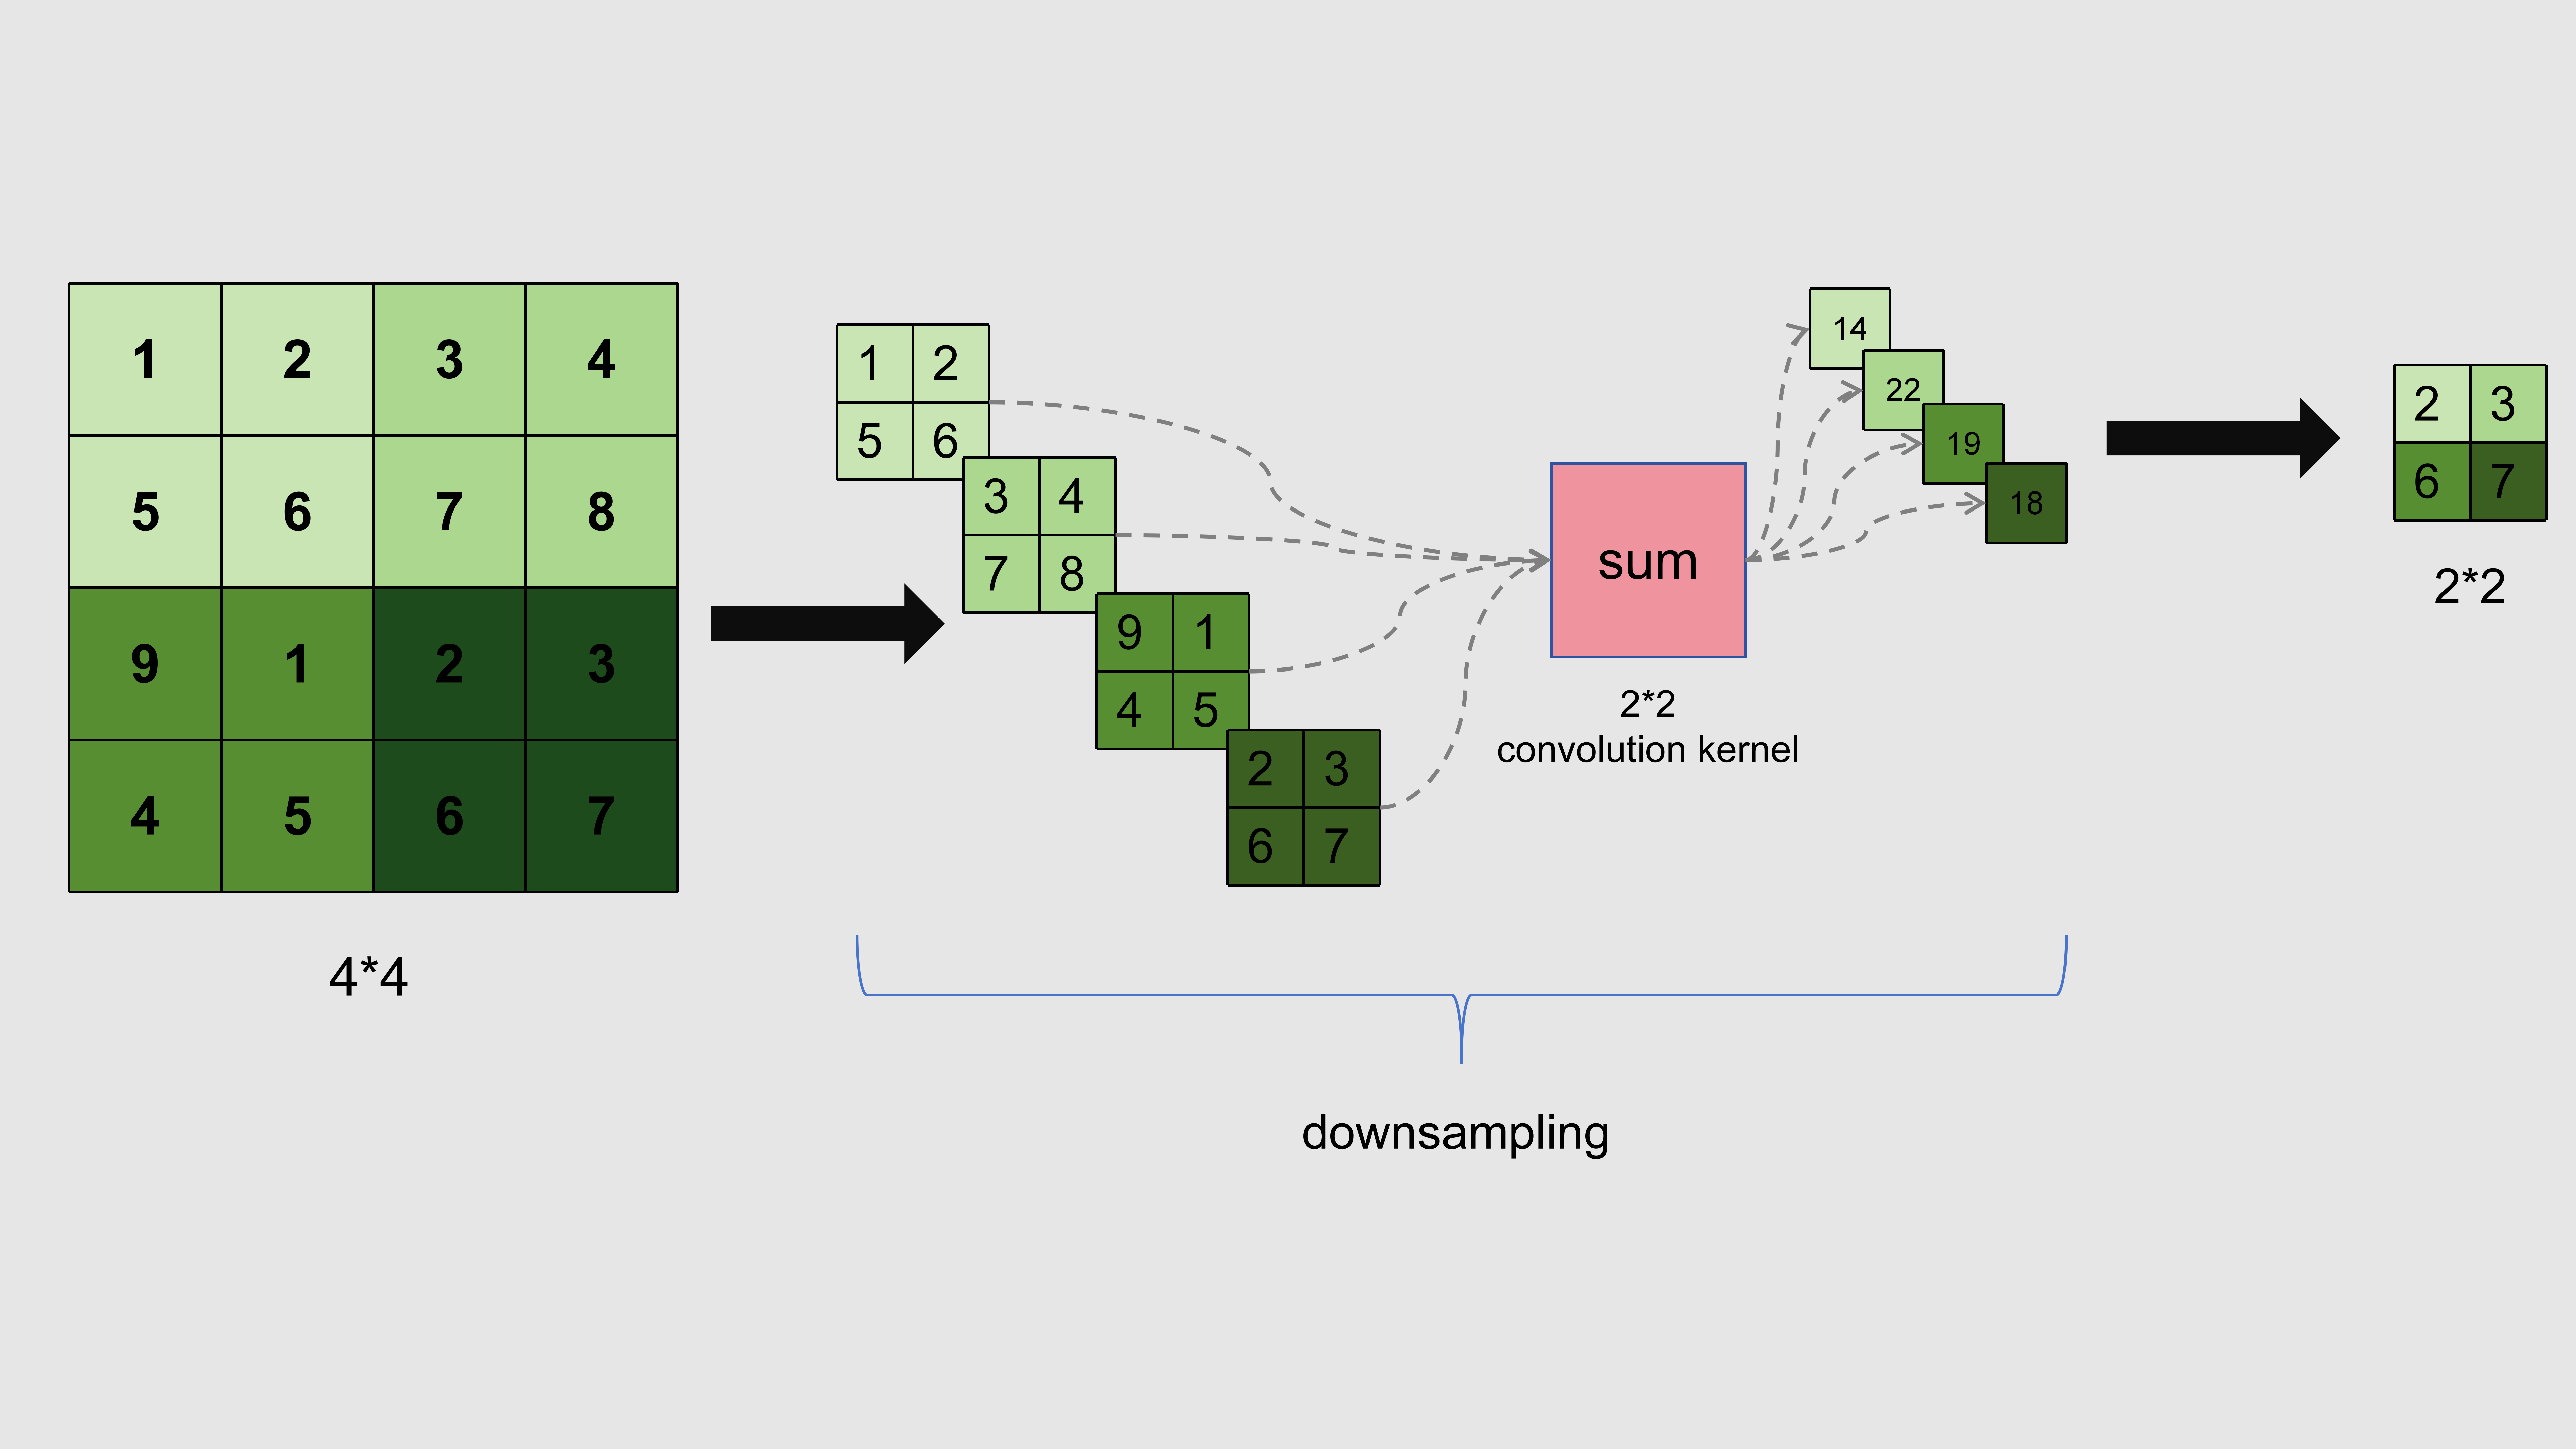
\includegraphics[width=0.75\linewidth]{figures_plus/拉普拉斯.png}
    \caption{}
    \label{fig:enter-label}
\end{figure}

\vspace{0.5em}
\textbf{2.Gaussian Decomposition}

Similar to the input image, each weight map is processed into a multi-scale version by Gaussian pyramid decomposition\textsuperscript{\cite{olkkonen1996gaussian}}. The Gaussian decomposition smoothes the weight maps and reduces the drastic changes in the weight maps at the boundaries, thus avoiding the introduction of artifacts in the fusion process.

\vspace{0.5em}
\textbf{3.Hierarchical Integration}

The fusion of the input image and the weight map is performed at each layer of the Laplace pyramid and Gaussian pyramid, respectively. The specific formulas are as follows:
\[R_l(x, y) = \sum_{k=1}^{K} G_l \{ \bar{W}^k(x, y) \} L_l \{ I_k(x, y) \}\]

Where:

\begin{itemize}[itemindent=2em]
    \item $L_{l}$ and $G_{l}$ denote the Laplace and Gaussian decompositions of the input and weight maps, respectively, at layer l.
\end{itemize}

\vspace{0.5em}
\textbf{4.Reconstruction of Results}

The fused results of all layers are reconstructed from the bottom up to obtain the final enhanced image. This method ensures that the fused image retains high-frequency details while providing a natural global distribution of brightness and contrast.

\subsection{Model Brought In}

After constructing the underwater image enhancement framework, we input the experimental data into the system to generate and visualize the enhanced image (as shown below). The results show significant improvements in overall clarity, contrast, and detail reproduction. Additionally, the color naturalness has been better restored, effectively addressing the blurring and color distortion caused by scattering and absorption.

\begin{figure}[htbp]
    \centering
    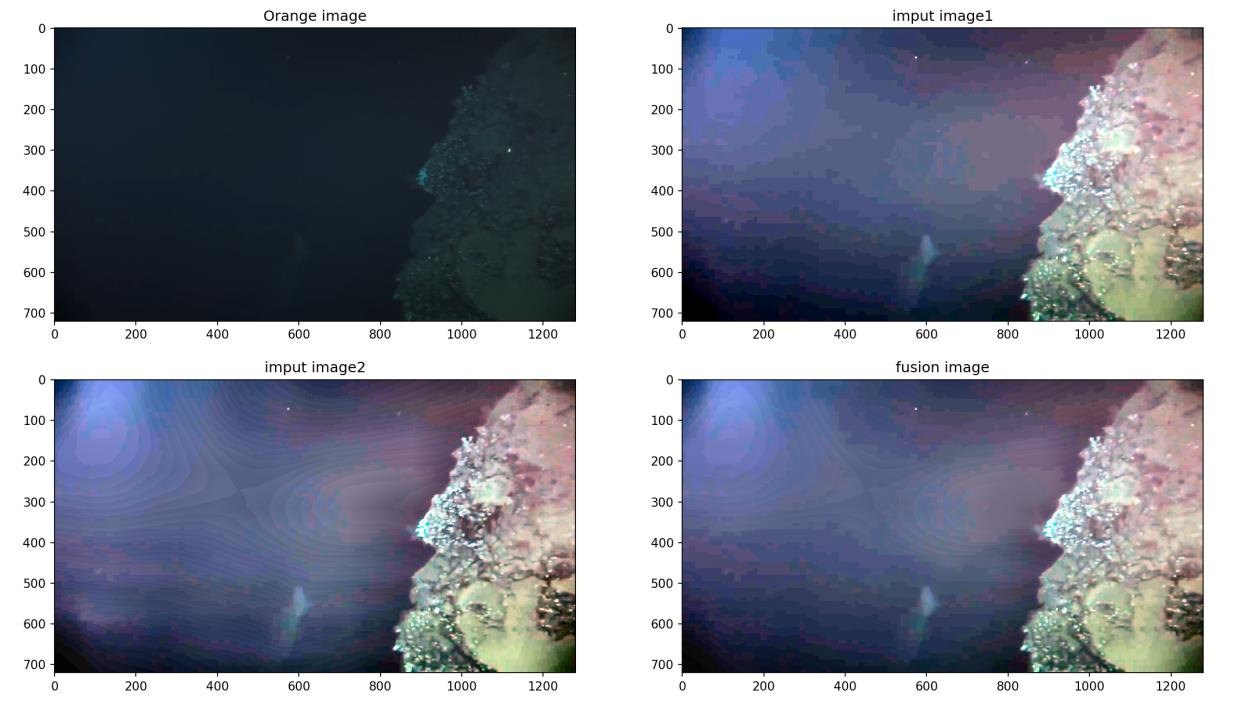
\includegraphics[width=0.9\linewidth]{figures_plus/可视化对比.png}
    \caption{}
    \label{fig:enter-label}
\end{figure}

In order to quantitatively assess the quality of the enhanced images, the Peak Signal to \textbf{Noise Ratio (PSNR)}, the \textbf{Underwater Image Quality Metrics (UIQM)} and the \textbf{Underwater Contrast and Color Enhancement Quality Metrics (UCIQE)} were calculated. The results are 27.32, 42.73 and 92.7, respectively.

\vspace{0.5em}
\textbf{PSNR:}

PSNR is used to measure the signal-to-noise ratio of an image, and a higher value indicates that the enhanced image has less distortion compared to the ideal image. From the results, the PSNR of 27.32 shows that the enhanced image has better performance in detail reproduction and the noise level is effectively controlled.

\vspace{0.5em}
\textbf{UCIQE:}

The UCIQE focuses on evaluating color uniformity, contrast, and saturation in underwater images. 42.73 of the UCIQE results show that the enhanced images have a significant advantage in terms of color balance and contrast enhancement, as well as more natural tonal transitions and a significant improvement in color cast.

\vspace{0.5em}
\textbf{UIQM}

The UIQM is a comprehensive underwater image quality metric, which includes the evaluation of contrast, color tone and sharpness. The UIQM result of 92.7 shows that the enhanced image has excellent quality in several dimensions, especially in the blurring of details, which is a common Question in underwater imaging.

That is, the effect of my image enhancement framework is better, after that we input the contents of Annex 2 into the model according to the requirements of the topic, and calculate the PSNR, UCIQE, UIQM of the obtained image, and output it to the required file.

\begin{table}[h!]
\centering
\resizebox{0.65\textwidth}{!}{ % 调整表格宽度为页面宽度的 75%，高度自动按比例缩放
\begin{tabular}{lccc}
\toprule
\textbf{Image File Name} & \textbf{PSNR} & \textbf{UCIQE} & \textbf{UIQM} \\ % 表头部分
\midrule
test\_001.png & 27.79328 & 39.77014 & 69.62394 \\ % 数据行
test\_002.png & 28.93661 & 37.13202 & 32.8004  \\
test\_003.png & 27.73244 & 41.95226 & 44.07396 \\
test\_004.png & 28.26598 & 44.33939 & 104.5923 \\
test\_005.png & 28.38353 & 28.08084 & 32.93351 \\
test\_006.png & 27.18512 & 39.14769 & 33.17518 \\
test\_007.png & 27.90435 & 33.87115 & 51.66059 \\
test\_008.png & 27.81145 & 33.16115 & 36.77311 \\
test\_009.png & 27.68675 & 29.88153 & 53.67291 \\
test\_010.png & 27.58939 & 34.6082  & 57.60875 \\
test\_011.png & 27.32634 & 29.99883 & 46.32982 \\
\bottomrule
\end{tabular}
}
\caption{} % 添加表格标题
\label{tab:your_label} % 添加表格标签供引用
\end{table}

%%%%%%%%%%%%%%%%%%%%%%%%%%%%%%%%%%%%%%%%%%%%%%%%%%%%%%%%%%%%%
\newpage
\section{Solution of Problem 5}

In underwater image enhancement research, specific scene enhancement techniques and single enhancement techniques for complex scenes each have their advantages and limitations. Specific scene enhancement techniques are typically designed for certain types of underwater environments, providing better results under specific conditions, while complex scene enhancement techniques are intended for more dynamic and challenging environments, with greater adaptability. Below is a detailed comparison of these techniques.

\subsection{Scene-Specific Enhancement Techniques}

Scene-specific enhancement techniques are optimized for particular underwater environments and can provide excellent results when applied to these specific conditions. Common scene-specific enhancement techniques include:

\textbf{Color Restoration}

\begin{itemize}[itemindent=2em]
    \item Scene: Shallow waters or clear environments.

    \item Technique: Restoring color components in images, particularly considering the light absorption characteristics in underwater environments (e.g., restoration methods based on dark channel priors).

    \item  Advantages: Effective at recovering colors in shallow waters and providing more natural visual effects.

    \item  Limitations: Less effective in deep or highly turbid waters where red light components are largely absorbed, leading to significant color distortion.
\end{itemize}

\textbf{Dehazing}

\begin{itemize}[itemindent=2em]
    \item Scene: Waters with moderate turbidity or shallow water environments.

    \item Technique: Removing haze and suspended particles in the water to enhance image clarity.

    \item  Advantages: Significantly improves the clarity of images, especially for medium turbidity waters.

    \item  Limitations: Less effective in deep or severely polluted water environments where the haze or scattering is more intense.
\end{itemize}

\textbf{Contrast Enhancement}

\begin{itemize}[itemindent=2em]
    \item Scene: Environments with insufficient lighting or low contrast.

    \item Technique: Applying histogram equalization or adaptive contrast enhancement to improve image contrast and highlight details.

    \item  Advantages: Improves the visibility of details, particularly in low-light conditions.

    \item  Limitations: Excessive enhancement can introduce noise, especially in low-quality images.
\end{itemize}

\textbf{Denoising}

\begin{itemize}[itemindent=2em]
    \item Scene: Noisy underwater images, particularly in environments with high pollution.

    \item Technique: Using methods like median filtering or bilateral filtering to remove noise.

    \item  Advantages: Effectively removes noise and preserves image details.

    \item  Limitations:Denoising can result in the loss of some fine details, particularly when noise levels are high.
\end{itemize}

\subsection{Complex Scene Single Enhancement Techniques}

Complex scene enhancement techniques are used for more dynamic, unpredictable underwater environments where conditions vary significantly. These techniques tend to be more adaptable, addressing multiple challenges in complex water environments. Common single enhancement techniques for complex scenes include:

\textbf{Deep Learning-Based Enhancement Techniques}

\begin{itemize}
    \item Scene: Suitable for a variety of challenging underwater environments, including low light, deep water, and polluted waters.

    \item Technique: Using deep neural networks (e.g., GANs, U-Net) to automatically learn image features and enhance images.

    \item Advantages: Capable of addressing multiple issues like dehazing, color restoration, and denoising, and doesn't require manual feature engineering.

    \item Limitations: Requires a large amount of training data, high computational resources, and may have high latency in real-time applications.
\end{itemize}

\textbf{Underwater Image Restoration}

\begin{itemize}
    \item Scene: Suitable for deep water or environments with severe light attenuation.

    \item Technique: Using physical models to estimate and restore underwater image distortion due to scattering and absorption.

    \item Advantages: Can restore color distortion and image details lost in deep waters where light is significantly absorbed.
    
    \item Limitations: Requires accurate underwater optical models and knowledge of the water's optical properties, which may not always be available.
\end{itemize}

\textbf{Multi-Scale Enhancement}

\begin{itemize}
    \item Scene: Environments with significant variations in light and water quality, such as turbid waters or highly dynamic water conditions.

    \item Technique: Using multi-scale convolutional neural networks (MS-CNN) or image pyramids to process image information at different scales.

    \item Advantages: Can capture details at multiple levels and enhance the overall appearance of the image.
    
    \item Limitations: High computational cost, and may produce artifacts when dealing with high dynamic range images.
\end{itemize}

\subsection{Feasibility Recommendations for Underwater Visual Enhancement in Practical Applications}

\subsection{Shallow Water and Clear Water Environments}

\begin{itemize}
    \item Recommendation: Use simple techniques such as color restoration, contrast enhancement, and basic denoising.

    \item Rationale: Shallow waters generally have good lighting and clear water, so simple enhancement methods can significantly improve image quality.

    \item Specific Approach:
        \begin{itemize}
            \item \textbf{Color restoration based on dark channel priors} can restore the lost color components, especially for shallow water images.

            \item \textbf{Contrast enhancement} (e.g., histogram equalization) can improve detail visibility, especially in well-lit waters.
        \end{itemize}
\end{itemize}

\subsection{Deep Water and Low-Light Environments}

\begin{itemize}
    \item Recommendation: Use deep learning-based enhancement methods or multi-scale enhancement techniques.

    \item Rationale: Deep water environments suffer from severe light attenuation, where simple enhancement techniques are insufficient. Deep learning methods can automatically learn features of the underwater environment and enhance images.

    \item Specific Approach:
        \begin{itemize}
            \item Use \textbf{GANs} or \textbf{U-Net} networks for image enhancement, restoring both color and fine details.

            \item  Apply \textbf{multi-scale convolutional networks} to handle different levels of details and improve image quality across varying depths and water conditions.
        \end{itemize}
\end{itemize}

\subsection{Turbid or Highly Polluted Water Environments}

\begin{itemize}
    \item Recommendation: Combine underwater image restoration based on physical models with deep learning-based denoising.

    \item Rationale: In turbid or highly polluted water, traditional enhancement methods may not be sufficient to recover image details. Combining restoration techniques with deep learning can effectively recover images.

    \item Specific Approach:
        \begin{itemize}
            \item Use \textbf{underwater image restoration} algorithms based on optical models to compensate for light scattering and absorption.

            \item Apply \textbf{denoising neural networks} (e.g., U-Net) to remove noise and recover fine details from polluted water images.
        \end{itemize}
\end{itemize}

\subsection{Real-Time Applications with High Performance Requirements}

\begin{itemize}
    \item Recommendation: Prioritize low-computation methods such as basic color restoration, dehazing, and denoising.

    \item Rationale: Real-time applications require fast processing, and deep learning-based methods might not meet latency requirements. Therefore, simple techniques that provide faster processing times are preferable.

    \item Specific Approach:
        \begin{itemize}
            \item \textbf{Dehazing algorithms} based on dark channel priors can quickly improve image visibility in low-light conditions.

            \item \textbf{Color restoration} methods and \textbf{denoising algorithms} (e.g., median filtering) can be efficiently implemented for real-time applications.
        \end{itemize}
\end{itemize}

\subsection{Conclusion}

\begin{itemize}
    \item \textbf{Scene-Specific Enhancement Techniques} are well-suited for simpler, more stable environments and can significantly improve image quality with minimal computational cost. These methods are best applied in clear waters or shallow environments where the challenges are mainly related to color distortion, low contrast, or slight noise.

    \item \textbf{Complex Scene Single Enhancement Techniques} are more suited to dynamic and unpredictable underwater environments, such as deep or polluted waters. These methods are generally more computationally intensive but provide greater adaptability and better handling of varied water conditions.

    \item \textbf{In practical applications}, the selection of enhancement techniques should depend on the specific underwater environment, available computational resources, and real-time processing requirements. Often, a combination of techniques tailored to the scene’s characteristics will provide the most effective solution for underwater visual enhancement.
\end{itemize}

%%%%%%%%%%%%%%%%%%%%%%%%%%%%%%%%%%%%%%%%%%%%%%%%%%%%%%%%%%%%%
\newpage
\section{Strengths and Weakness}

\subsection{Advantages of the Model}
\begin{itemize}[itemindent=2em]
\item \textbf{Solid theoretical foundation:} The model is based on the underwater optical transmission model, considering light absorption and scattering effects, offering a more accurate simulation of underwater image degradation.

\item \textbf{Parametric design:} The model is tunable, with key optical parameters such as absorption coefficients, scattering coefficients, and background light intensity, allowing it to adapt to different water conditions and degradation types.

\item \textbf{Multi-level enhancement strategy:} The model uses hierarchical enhancement techniques\textsuperscript{\cite{wang2008optimizing}} (e.g., histogram equalization, color correction, Laplace sharpening) to improve image quality by addressing brightness, color, and sharpness degradation.

\item \textbf{Perfect evaluation system:} Metrics like PSNR, UCIQE, and UIQM provide a clear, quantitative measure of enhancement performance, aiding model optimization.

\item \textbf{Visual display:} The model provides visual representations of prediction errors, offering insights for further optimization and a clearer understanding of model performance.

\end{itemize}

\subsection{ Disadvantages of the Model}

\begin{itemize}[itemindent=2em]

\item  \textbf{Limitations of simplifying assumptions:} The model ignores multiple scattering effects and dynamic water conditions to reduce complexity, limiting its application in more complex underwater environments.

\item  \textbf{Recovery is dependent on parameterization:}  The model's effectiveness relies heavily on precise parameter estimation (e.g., water depth, background light intensity). Large deviations in parameter values may affect recovery performance.

\item \textbf{Insufficient scene adaptation:} Some enhancement methods may not perform well in extreme conditions, such as high turbidity or low-light environments, requiring further algorithm robustness improvements.

\item \textbf{Higher computational complexity:} For large-scale image data, especially for models incorporating multiple enhancement techniques, computation time may be a limiting factor and is not suitable for real-time processing scenarios.

\end{itemize}

\subsection{Future Outlook}

These models can be generalized and applied in several domains and scenarios:

\begin{itemize}[itemindent=2em]
    \item \textbf{Dynamic Water Environment Modeling:} Incorporating dynamic water conditions, such as fluctuations and suspended particles, could improve model adaptability and robustness in complex underwater environments.

    \item \textbf{Multimodal Information Integration:} Combining optical images with acoustic signals and laser scanning data could lead to more comprehensive enhancement models for improved image quality.

    \item \textbf{Real-Time Processing Optimization: } Efficient algorithm optimization and hardware acceleration (e.g., GPU computing) could address the computational challenges, enabling real-time processing for practical applications.

    \item \textbf{Standardized Datasets and Evaluation System: } Creating open standard datasets for underwater image degradation and enhancement and a unified evaluation system could support model generalization and standardization.

    
\end{itemize}

%%%%%%%%%%%%%%%%%%%%%%%%%%%%%%%%%%%%%%%%%%%%%%%%%%%%%%%%%%%%%
%% 参考文献
\newpage

\nocite{*}
\bibliographystyle{gbt7714-numerical}  % 引用格式

\bibliography{ref.bib}  % bib源

%%%%%%%%%%%%%%%%%%%%%%%%%%%%%%%%%%%%%%%%%%%%%%%%%%%%%%%%%%%%%
%% 附录
% \appendix
% \section*{附录一}
% \addcontentsline{toc}{section}{附录一}

% \lstinputlisting[language=Python]{code/Problem 1.py}

% \newpage
% \appendix
% \section*{附录二}
% \addcontentsline{toc}{section}{附录二}

% \lstinputlisting[language=Python]{code/Problem 2.py}

% \newpage
% \appendix
% \section*{附录三}
% \addcontentsline{toc}{section}{附录三}

% \lstinputlisting[language=Python]{code/Problem 3.py}

% \newpage
% \appendix
% \section*{附录四}
% \addcontentsline{toc}{section}{附录四}

% \lstinputlisting[language=Python]{code/Problem 4.py}


\end{document}

